%%%%%%%%%%%%%%%%%%%%%%%%%%%%%%%%%%%%%%%%%%%%%%%%%%%%%%%%%%%%%%%%%%%
%                                                                 %
%                            ROOT FILE                            %
%                                                                 %
%%%%%%%%%%%%%%%%%%%%%%%%%%%%%%%%%%%%%%%%%%%%%%%%%%%%%%%%%%%%%%%%%%%
%
%  Run LaTeX or pdfLaTeX on this file to produce your thesis.
%  To produce the abstract title page followed by the abstract,
%  see the file abstitle-phd.tex or abstitle-mas.tex.
%
%%%%%%%%%%%%%%%%%%%%%%%%%%%%%%%%%%%%%%%%%%%%%%%%%%%%%%%%%%%%%%%%%%%

\documentclass[chap]{thesis}

\usepackage{url}
\usepackage{mdframed}
\usepackage{amsmath}
\usepackage{amssymb}
\usepackage{color}
\usepackage{proof}
\usepackage{bussproofs}
\usepackage{graphicx}
\usepackage{booktabs}
\usepackage{paralist}
\usepackage{comment}
\usepackage{lmodern,textcomp}
\usepackage{subfigure}
\usepackage[usenames,dvipsnames,svgnames,table]{xcolor}


\newcommand{\E}{\ensuremath{\mathcal{E}}}
\newcommand{\F}{\ensuremath{\mathbf{F}}}
\newcommand{\SEQ}{\ensuremath{\mathit{SEQ}}}
\newcommand{\N}{\ensuremath{\mathbb{N}}}

\newcommand{\Fecon}{\ensuremath{\F_{\!\mathit{econ}}}}
\newcommand{\M}{\ensuremath{\mathcal{M}}}

\newcommand{\lmethod}[1]{%
  \mbox{\textbf{#1}}}

\newcommand{\lsort}[1]{%
  \ensuremath{\mbox{\textsf{#1}}}}
\newcommand{\defsort}[2]{%
  \newcommand{#1}{\lsort{#2}}}
\defsort{\Action}{Action}
\defsort{\Time}{Time}
\defsort{\Self}{Self}

\defsort{\Agent}{Agent}
\defsort{\Entrant}{Entrant}
\defsort{\ActionType}{ActionType}
\defsort{\Moment}{Moment}
\defsort{\Boolean}{Formula}
\defsort{\PayOut}{PayOut}
\defsort{\Fluent}{Fluent}
\defsort{\Event}{Event}
\defsort{\Object}{Object}
\defsort{\RealTerm}{RealTerm}

\defsort{\Numeric}{Numeric}
\defsort{\Number}{Number}
\defsort{\Trolley}{Trolley}
\defsort{\Track}{Track}
\defsort{\Moveable}{Moveable}


\newcommand{\lsymbol}[1]{%
  \ensuremath{\mathit{#1}}}
\newcommand{\defsymbol}[2]{%
  \newcommand{#1}{\lsymbol{#2}}}
\defsymbol{\action}{action}
\defsymbol{\initially}{initially}
\defsymbol{\holds}{holds}
\defsymbol{\happens}{happens}
\defsymbol{\clipped}{clipped}
\defsymbol{\initiates}{initiates}
\defsymbol{\terminates}{terminates}
\defsymbol{\prior}{prior}
\defsymbol{\interval}{interval}

\defsymbol{\vicinity}{vicinity}

\newcommand{\lconstant}[1]{%
  \ensuremath{\mbox{\textsf{#1}}}}
\newcommand{\defconstant}[2]{%
  \newcommand{#1}{\lconstant{#2}}}
\defconstant{\Enter}{Enter}
\defconstant{\StayOut}{StayOut}
\defconstant{\Fight}{Fight}
\defconstant{\Acquiesce}{Acquiesce}
\defconstant{\cs}{cs }
\newcommand{\trackA}{\ensuremath{track_1}}
\newcommand{\trackB}{\ensuremath{track_2}}

\newcommand{\lmodality}[1]{%
  \ensuremath{\mathbf{#1}}}
\newcommand{\defmodality}[2]{%
  \newcommand{#1}{\lmodality{#2}}}
\defmodality{\common}{C}
\defmodality{\knows}{K}
\defmodality{\believes}{B}
\defmodality{\perceives}{P}
\defmodality{\mental}{M}
\defmodality{\requests}{R}


\defmodality{\desires}{D}
\defmodality{\intends}{I}
\defmodality{\says}{S}
\defmodality{\ought}{O}


\newcommand{\EC}{\ensuremath{\mathcal{EC}}}
\newcommand{\CEC}{\ensuremath{\mathcal{CEC}}}
\newcommand{\DCEC}{\ensuremath{\mathcal{DCEC}}}

\newcommand{\lif}{\rightarrow}
\newcommand{\liff}{\leftrightarrow}
\newcommand{\sep}{\ \lvert \ }


\newcommand{\DDE}{\ensuremath{\mathcal{{DDE}}}}
\newcommand{\DTE}{\ensuremath{\mathcal{{DTE}}}}
\newcommand{\type}[1]{\textsf{#1}}

\newcommand{\Intends}{\ensuremath{\mathbf{I}}}
\newcommand{\Believes}{\ensuremath{\mathbf{B}}}

\newcommand{\Knows}{\ensuremath{\mathbf{K}}}

\newtheorem{assumption}{Assumption}

\defsort{\Table}{Table}
\defsort{\Block}{Block}
\defsort{\Surface}{Surface}
\defsort{\Goal}{Goal}

\defsymbol{\on}{on}
\defsymbol{\clear}{clear}
\defsymbol{\stack}{stack}
\defsymbol{\unstack}{unstack}
\defsymbol{\inRoom}{inRoom}
\defsymbol{\position}{position}

\defsymbol{\setGoal}{setGoal}
\defsymbol{\removeGoal}{removeGoal}
\defsymbol{\goal}{goal}

\defconstant{\ctable}{$\mathit{table}$}
\defconstant{\ablock}{$A$}
\defconstant{\bblock}{$B$}
\defconstant{\cblock}{$C$}
\defconstant{\humana}{$h_1$}
\defconstant{\humanb}{$h_2$}
\defconstant{\cir}{$\mathit{cais}$}

%% CAIS %%
\defsymbol{\point}{point}
\defsymbol{\register}{register}
\defsymbol{\deregister}{deregister}
\defsymbol{\inCAIS}{inCAIS}
\defsymbol{\distance}{distance}

%% Sticky Notes
\defsort{\Color}{Color}
\defsort{\Note}{Note}

\defsymbol{\onScreen}{onScreen}
\defsymbol{\onDevice}{onDevice}
\defsymbol{\isColor}{isColor}
\defsymbol{\pickUp}{pickUp}
\defsymbol{\putDown}{putDown}
\defsymbol{\delete}{delete}

%%%%%

\newcommand\blfootnote[1]{%
  \begingroup
  \renewcommand\thefootnote{}\footnote{#1}%
  \addtocounter{footnote}{-1}%
  \endgroup
}

%\newcommand{\checkmark}{\color{black}\checkmark\color{black}}

% Uncomment the following if you want centered-lined captions:
%\captionsetup{format=plain,justification=centering}


%\includeonly{rpichap1}  % use \includeonly to process only
                         % the file(s) listed inside the braces

\begin{document}

% Use the appropriate example title page.  A senior thesis
% can be set by changing the thesis name in rpititle-mas.tex.

%%%%%%%%%%%%%%%%%%%%%%%%%%%%%%%%%%%%%%%%%%%%%%%%%%%%%%%%%%%%%%%%%%% 
%                                                                 %
%                            TITLE PAGE                           %
%                            PhD Thesis                           %
%                                                                 %
%%%%%%%%%%%%%%%%%%%%%%%%%%%%%%%%%%%%%%%%%%%%%%%%%%%%%%%%%%%%%%%%%%% 
%  This file produces the title page, copyright page (if requested)
%  and the Table of Contents, List of Figures and List of Tables.
% 
%  To produce the abstract title page followed by the abstract,
%  see the template file, "abstitle-phd.tex"
%%%%%%%%%%%%%%%%%%%%%%%%%%%%%%%%%%%%%%%%%%%%%%%%%%%%%%%%%%%%%%%%%%%
    
% Supply information for use on title page:
%   
\thesistitle{\bf Building Cognitive and Immersive Systems:\\
Architecture, Implementation, and Formalization}      
\author{Matthew Peveler}
\degree{Doctor of Philosophy}        
\department{Computer Science} % provide your area of study here; e.g.,
%  "Mechanical Engineering", "Nuclear Engineering", "Physics", etc.   
     
\signaturelines{5}   %max number of signature lines is 7        
\thadviser{Selmer Bringsjord}
\cothadviser{Hui Su} % If you have 2 thesis advisers
\memberone{Carlos Varela}        
\membertwo{Bolesław Szymański}
\memberthree{Jeff O. Kephart}

\submitdate{[December 2020]\\ Submitted December 2020}
\copyrightyear{2020}   % if omitted, current year is used.        

% Print titlepage and other prefatory material:
%    
\titlepage     
\copyrightpage         % optional           
\tableofcontents        
\listoftables          % required if there are tables
\listoffigures         % required if there are figures


   % titlepage material for PhD thesis
%%%%%%%%%%%%%%%%%%%%%%%%%%%%%%%%%%%%%%%%%%%%%%%%%%%%%%%%%%%%%%%%%%%% 
%                                                                 %
%                         ACKNOWLEDGEMENT                         %
%                                                                 %
%%%%%%%%%%%%%%%%%%%%%%%%%%%%%%%%%%%%%%%%%%%%%%%%%%%%%%%%%%%%%%%%%%% 
 
\specialhead{ACKNOWLEDGMENT}
 
I would like to thank this is a sentence to take up space and look
like text.  This is a sentence to take up space and look like text.
This is a sentence to take up space and look like text.  This is a
sentence to take up space and look like text.  This is a sentence to
take up space and look like text.  This is a sentence to take up space
and look like text.
 
This sentence, meant to take up space, also helped to take up space
and look like text.  This is a sentence to take up space and look like
text.  This is a sentence to take up space and look like text.  This
is a sentence to take up space and look like text.  This is a sentence
to take up space and look like text.  This is a sentence to take up
space and look like text.  This is a sentence to take up space and
look like text.  This is a sentence to take up space and look like
text.  This is a sentence to take up space and look like text.
 
This is a sentence to take up space and look like text.
This is a sentence to take up space and look like text.
This is a sentence to take up space and look like text.
 
This is a sentence to take up space and look like text.
This is a sentence to take up space and look like text.
This is a sentence to take up space and look like text.
  % include for acknowledgements

%%%%%%%%%%%%%%%%%%%%%%%%%%%%%%%%%%%%%%%%%%%%%%%%%%%%%%%%%%%%%%%%%%% 
%                                                                 %
%                            ABSTRACT                             %
%                                                                 %
%%%%%%%%%%%%%%%%%%%%%%%%%%%%%%%%%%%%%%%%%%%%%%%%%%%%%%%%%%%%%%%%%%% 
 
\specialhead{ABSTRACT}
 


% 1. Introduction
\chapter{Introduction, Background, and Motivation}\label{chap:introduction}

% 1. Introduction
\section{Introduction}

In contemporary AI research, especially as devoted to decision
support, the challenge is often taken to be that of providing AI
support to a single human on their own personal device. However, much
human problem solving is fundamentally social, in that a group of
people must work together to solve a problem, and must rely upon
machine intelligence that is itself highly diverse.  Examples of such
activities include: hiring a person into a university or company,
tackling an emergency crisis like a major water pipeline break,
planning an intricate medical operation, and deciding which companies
to merge with or acquire.  Motivated by such challenges, we are
interested in how an artificial agent --- embedded in a
social-collaboration environment like an immersive room --- can, on
the spot, help a group of human participants.

%%%%%%%%%%%%%%%%%%%%%%%%%%%%%%%%%%%%%%%%%%%%%%%%%%%%%%%%%%%%%%%%%%%%%%
\begin{figure}
\centering
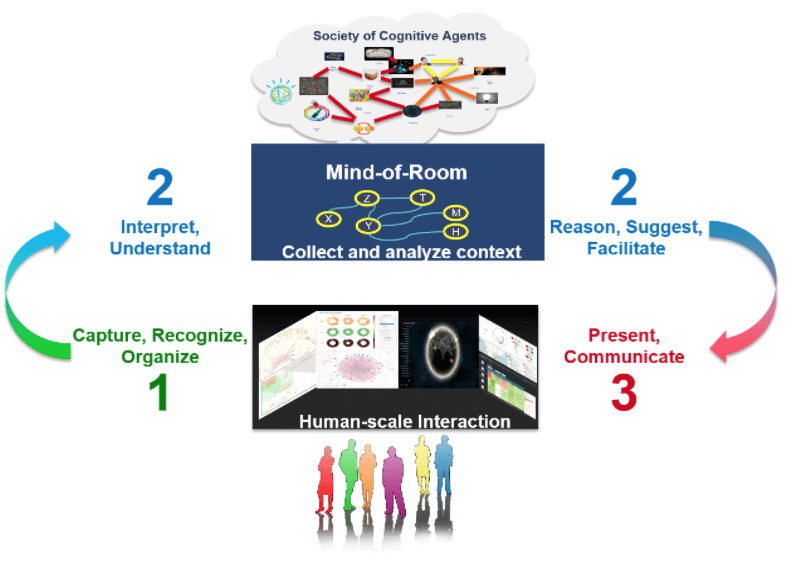
\includegraphics[width=0.5\columnwidth]{chapters/01_introduction/figures/cisl-cycle-graphic.png}
\caption{The flow of information through the elements of a cognitive and immersive system.}
\label{fig:cycle-cais}
\end{figure}
%%%%%%%%%%%%%%%%%%%%%%%%%%%%%%%%%%%%%%%%%%%%%%%%%%%%%%%%%%%%%%%%%%%%%%

We first introduce the notion of a \emph{cognitive and immersive
  system} (CAIS), which comprises three elements linked in a cyclical
flow as shown in Figure \ref{fig:cycle-cais}.  The first element is
responsible for perception and sensing within the environment that
contains the human agents (such as a room). Percepts come courtesy of
a range of sensors, such as microphones and kinects. From these
percepts, we receive information such as what was said, where users
are in the room, etc. The second element, upon receiving that
information, is responsible for interpreting, understanding, and
executing on the basis of that data. In this process, the CAIS may
employ reasoners, planners, databases, etc.\ to drive its
execution. The third element displays both percepts and the results of
processing these percepts in rich, multi-modal ways, such as showing
content on displays or speaking to the users of the system. As part of
the operation of the CAIS, we expect that it has access both to local
modules, as well as is able to make use of external machines and
services that are well-suited to specific tasks or domains. Perhaps
most important to note here is that these external services may be
requested for and opened by users of the system, but that one
reasonably expects that a CAIS should be able to handle these things
in a meaningful and useful fashion.
%% MATT2:  Previous sentence quite hard to understand.  Pls rework.
An important part of our system is that there are overseeing AIs
(agents) operating at the system level that can use the rest of the
system to assist and aid the humans and other AIs that are operating
within.  Thus, the overarching architecture is neither fully
centralized nor fully distributed, but aims to combine the strengths
of both.

Stemming from this overseeing AI, being that it captures all that goes
on within a CAIS, we can look to realize a number of useful
capabilities and principles. Most important here is that these stem
from a rigorous formalization, not from an \textit{ad hoc}
process. From these formal requirements and formalized operations, we
explore how this then also enables our CAIS to possess deeper levels
of understanding of human agents within the room, operating at a
proper theory-of-mind level~\cite{premack_does_1978}, and makes
capable automated means of reasoning, planning, and plan recognition.
An example of this is shown in the following section, and further
explored in Chapter~\ref{chap:planning}, utilizing reasoning to
determine the knowledge and belief of agents, and plan recognition of
what agents are attempting to accomplish to provide meaningful
assistance.

This dissertation is divided into three major parts. The first part
consists of this chapter and deals with the high level goals we lay
out for cognitive-and-immersive systems. We present a motivating
example, and discuss at a high-level abstract view what an idealized
CAIS may be able to accomplish. The second part of the dissertation
concerns mplementation of a real-world CAIS, focusing on two novel
compoments that allow us to to achieve mechanisms being multi-modal
and multi-user without having the system then be constrained to one
specific type of use case or domain. This part is encapsulated in
Chapters 2, 3, and 4. For the third part, which makes up Chapters 5
and 6, we now provide a formalization for these sorts of systems,
stemming from the implmentation in part 2, and then look to see how we
can utilize this for tasks in reasoning, planning, and plan
recognition. Finally, we conclude the work with a summary of our
contributions and recognize promising avenues of future work that
exist.


% 3. Motivating Example
\subsection{Motivating Example}

In this section, we provide an overarching motivating example to help
illuminate the challenges we hope to solve within this work. To help further
ground the work, we present an example that could be commonplace within a joint
meeting space, and does not include a contrived setup.

Imagine that within a CAIS, there are three humans, Alvin, Betty, and Charlie,
who are all jointly working on a shared problem. Alvin and Betty are standing
next to each other, while Charlie stands apart. There is content on the screen
that relates to the problem. Betty looks at Alvin, then points at a particular
region of the screen. Alvin, seeing that Betty is looking at him, looks at her,
then follows to where she is pointing at the screen. Charlie is not looking at
either Alvin or Betty, nor at the region of screen that Betty is pointing at,
but instead at some other region of the screen. Betty gestures at the region of
the screen that she is pointing at, and the content changes in some way. Alvin,
who is following along the pointing and gesture, perceives both the gesture, and
the content change on the screen, while Charlie does not. Alvin then points to
the screen and makes a gesture, changing the content on the screen for a second
time. Betty perceives the pointing and gesture that Alvin does, while Charlie is
still oblivious to it. The time for this meeting concludes, and Betty might
reasonably ask "is everyone on the same page?". Neither Alvin or Betty are aware
that Charlie is not, while Charlie is unaware of the changed content. The
CAIS steps in, saying that no, Charlie is not on the same page, and that here
is a summary of the actions of Alvin and Betty for Charlie to catch him up,
covering the content that Alvin and Betty had both pointed at, as well as
the content that had changed on the screen.

From this example, we see that the CAIS must possess a number of sophisticated
pieces of machinery. For the physical space, the CAIS must possess the capacity
of knowing who is using the system, the physical actions that they
undertake, and what these agents might say. The CAIS then must possess the
capacity to display information to the human participants and speak to the
human participants. Finally, the CAIS must be able to connect the physical
actions of the humans, to that of the content that is being shown within the
space, such that it connects Betty gesturing at the screen with content under
that gesture.


% 2. Requirements of a CAIS
\section{Requirements of CAIS}\label{ref:requirements_cais}

It should be noted that for a CAIS to be considered a truly
``intelligent'' room, it is not sufficient that the room be
intelligent about, for example, search queries over a domain $D$; the
room should also be intelligent about cognitive states of agents in
the room and their cognitive states towards $D$.

Despite there being a significant amount of work done in building
intelligent environments (of varying levels of intelligence;
\cite{coen_design_1998,brooks_intelligent_1997,chan_review_2008}),
there is no formalization of what constitutes an intelligent room and
what separates it from an intelligent agent.  Though
\cite{coen_design_1998} briefly differentiates an intelligent room
from ubiquitous computing based on the non-ubiquity of sensors in the
former, there is not any formal or rigorous discussion of what
separates an intelligent room from a mobile robot that roams around
the room with an array of sensors. As far as we are aware, this work
is novel in its act of providing a characterization of what separates
an intelligent room from an intelligent agent.

The requirements in question are cognitive in nature and exceed
intelligent rooms with sensors that can answer queries over simple
extensional data (e.g.\ a room that can answer financial queries such
as \textit{``Show me the number of companies with revenue over X?''}).
At a high-level, we require two conditions below hold:

\begin{itemize}
    \item $\mathcal{C}$ \emph{Cognitive}: A CAIS should be able to
      help agents with cognitive tasks and goals.  For instance, a
      system that simply aids in querying a domain $D$ is not
      cognitive in nature; a system that knowingly aids an agent in convincing
      another agent that some state-of-affairs holds in $D$ is
      considered cognitive. (Please see the appendix for more
      discussion of our usage of the term ``cognitive.'')
    \item $\mathcal{I}$ \emph{Immersive}: There should be some
      attribute or property of a CAIS that is non-localized and
      distinguished from agents in the room.  Moreover, this property
      should be \textbf{common knowledge}.\footnote{For our purposes,
        common knowledge as defined in Chapter~\ref{chap:formalizing}
        is that all agents know this property, and know that all other
        agents know it.}  (Note: this is not easily achievable with a
      physical robot, and this condition differentiates a CAIS from a
      cognitive agent.)
\end{itemize}

While we believe that $\mathcal{C}$ is fully realizable and is
achieved as part of this dissertation, $\mathcal{I}$ is certainly far
more ambitious, given the high level of sophistication necessary for
an implementation that satisfies this condition. As such, we posit
that for a true formalization to hold any water, it must stem from the
implementation and not vice versa. In this way, we can ground our
formalization in a working system that can properly showcase both the
formalization and our technology.

\begin{comment}
\footnote{This condition may not strictly be realizable,
        but the goal is to at a minimum build systems that approach
        this ideal condition.}
\end{comment}


% 1. Overarching Goals


% 4. Colocated vs Distributed

\section{On Co-location vs Distributed Usage}

Before continuing, we would like to take a moment to discuss the
beliefs of co-location vs distributed usage of these sorts of
technologies. Within this work, we present, and focus on, a vision of
how such systems can be applied and help with co-located
participants. While we do believe that elements of this work can be
applied to a digital domain, doing so fundamentally changes the
paradigm of collaboration. When working together, we use the humans
%% MATT2:  "use the humans"?  Not sure what is meant here.  Pls
%% clarify, refine.  Thx.
utilize different levels of coupling, increasing or decreasing based
on the extent of communication that is required by the task at
hand~\cite{salvador_denver_1996,olson_distance_2000}. However, it is
important that coupling is not a static concept through a task, rather
that it is dynamic, changing through the lifetime of a
task~\cite{jakobsen_up_2014}.  Within this coupling, we see rise to a
concept of ``we-awareness" amongst
participants~\cite{greenberg_implications_2016}, as they utilize some
level of implicit understanding of verbal and non-verbal
communications. These concepts do not easily transfer to distributed
digital systems wherein participants are no longer standing next to
each other, rather sharing a ``space'' through interfaces like video
chat. Take for example pointing to something on a screen. With two
people standing next to each other, and one pointing at a shared
screen, we can make reasonable assumptions regarding the cognitive
states of agents, what they're perceiving, and also regarding what
they might believe about each other and what each other perceives.

Moving to the digital realm, these concepts cannot be immediately
recast as is, as one must first design the necessary mechanisms to
capture that information, transmit it to the other participants, and
to do so in such a way that the many rich and subtle parts of that
face-to-face interaction are not lost. Given the complexity of that
task, and the research area unto itself it would require, we do not
attempt to give the parallels here; we instead focus just on the topic
of handling the work in the co-located version only.


% 5. Contributions of the Dissertation


% 2. Technology of a Cognitive and Immersive System
\chapter{Technology for Cognitive and Immersive System}

% 1. Introduction
\section{Introduction}

In the previous chapter, we introduced the concept of cognitive and immersive
systems, and we laid out high-level ideals. As stated there, before we may turn
to the act of formalization, we first turn our attention to the creation of
the CAIS architecture, along with a real-world implementation. As stated before,
this implementation will help inform and establish the possibilities of our
formalization process. This process stems that building a CAIS brings to bear
many fields of research, such as computer vision, natural language processing,
reasoning, planning, operating in harmony. Recent advances in each allow us
to create something that can be used for a range of use cases and possibilities.
Su~\cite{su_cognitive_2017} articulated a vision of some of the complex use
cases in which these systems can be brought to tackle including language
learning, assisting in decision making, and data exploration. While we target
decision making here, the usages of this technology are as such more far reaching.

In this vein, we view that the CAIS must be targeted and utilize technologies
that can be applied across domains easily and quickly. Additionally, we readily
demand that the system be multi-user and multi-modal to achieve the level of
immersion required by our earlier principles. We find it important to note here
that we look to achieve our multi-modality such that each modality is available
to all users at all times. Finally, we aim that our CAIS should be easy to deploy
and utilize across domains. In this fashion, we aim to support a number of
environments that can contain differing capabilities and configurations. For
example, within the work for this dissertation, we deploy the CAIS to two
configurations, one a lab wall and the other a 360$^{\circ}$ screen, shown in
Figure~\ref{fig:cais_environments}. 

\begin{figure}
\centering
    \begin{subfigure}[b]{.47\linewidth}
        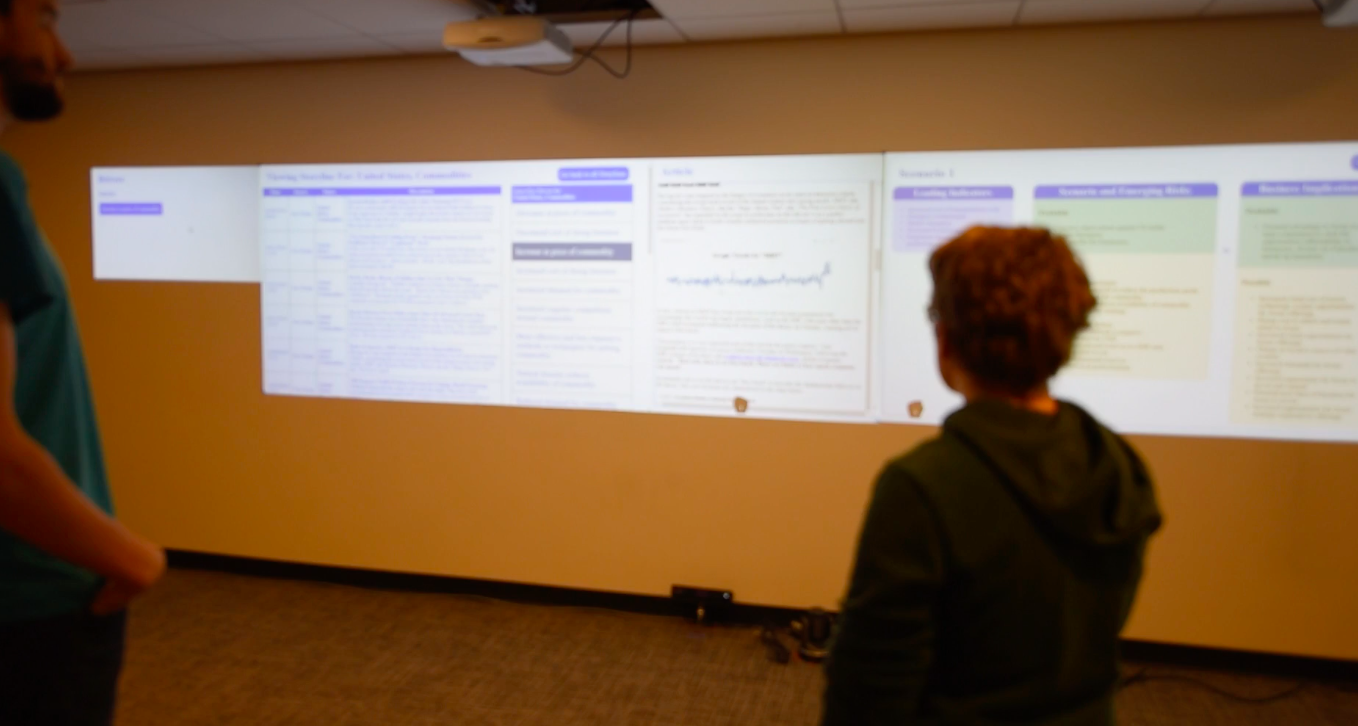
\includegraphics[width=\linewidth]{chapters/02_technology/figures/env_wall.png}
    \end{subfigure}
    \begin{subfigure}[b]{.48\linewidth}
        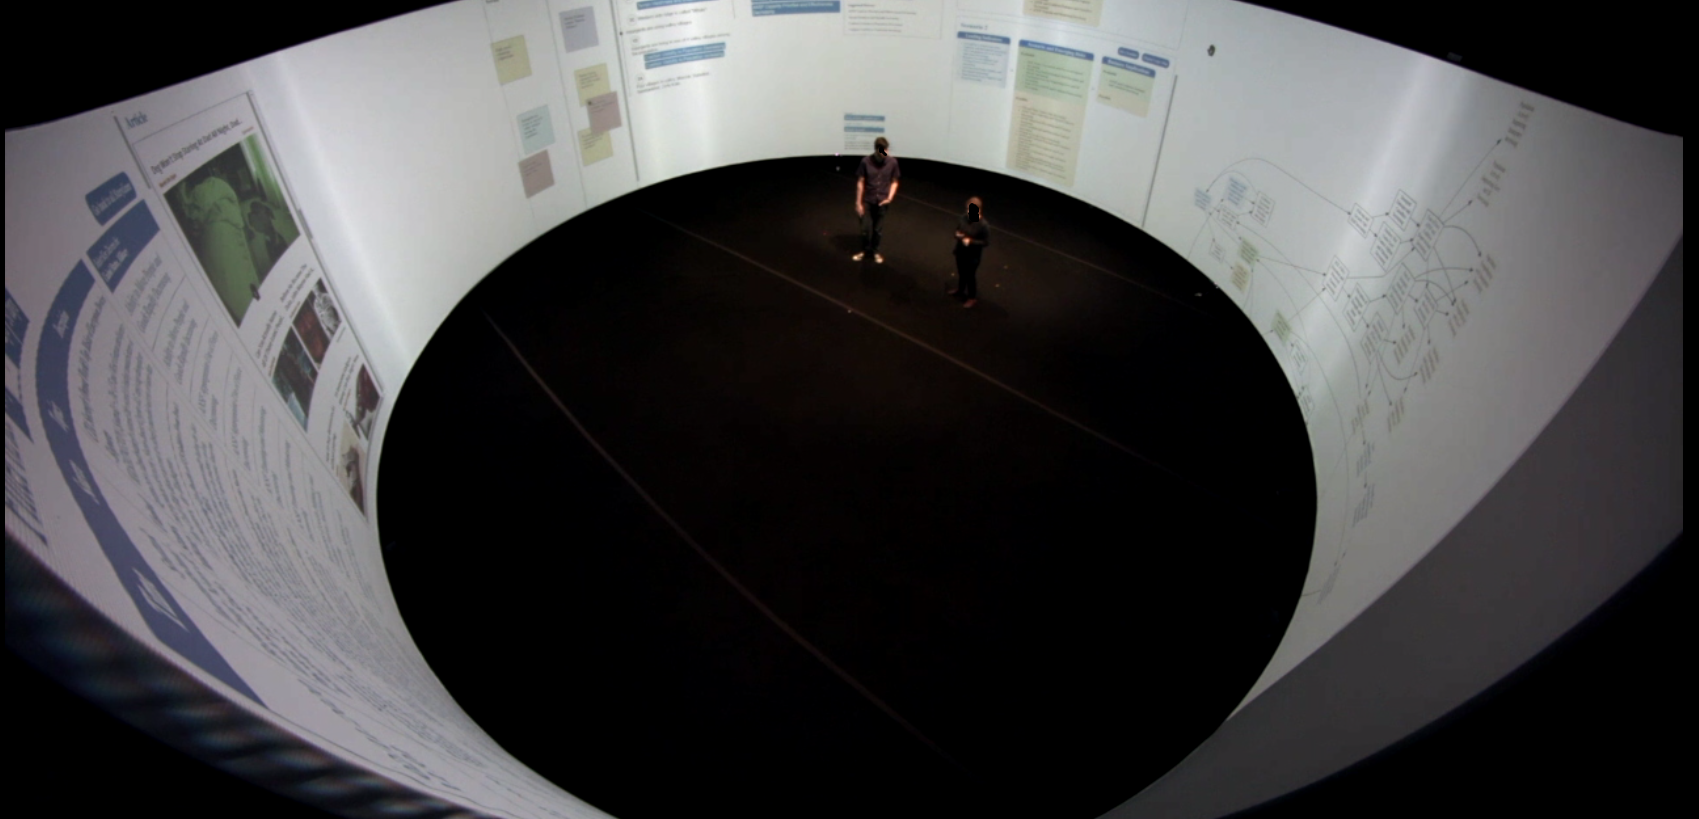
\includegraphics[width=\linewidth]{chapters/02_technology/figures/env_360.png}
    \end{subfigure}
    \caption{Two environments in which we deploy the CAIS, one a long flat wall and the other 360$^{\circ}$ screen.}
    \label{fig:cais_environments}
\end{figure}

% 2. Related Work
\section{Related Work}

There is a rich background of work for the design of multimodal systems, and more broadly the intelligent rooms
in which these systems are situated.

Historically, these systems have fallen into the category of ``smart rooms''
where multimodal input is much more of a necessity for more ``natural''
interaction than traditional desktop environments. In these multimodal
``smart rooms'', various efforts have been shown for picking up
where a user is pointing and using it in combination with
their voice to generate a command
\cite{bolt_put-that-there:_1980,carbini_wizard_2006,langner_multiple_2019,farrell_symbiotic_2016,kephart_embodied_2019}.
However, these systems hand-build their display layer and
content to embed the necessary instrumentation for combining speech
and gesture. Alternatively, \cite{coen_design_1998,brooks_intelligent_1997} demonstrate a system that
hooks into the X display server and could act on the content that was passed through
it from various applications, such as Netscape. While a very powerful approach, it
does not easily work across platforms, and that the security model of modern
applications such as Chrome renders the approach
increasingly impossible. Perhaps the most radical, \cite{roman_middleware_2002} propose an entire middleware infrastructure, similar to an OS,
to underpin these multimodal applications, but this approach
even more readily runs into the aforementioned bottleneck
in that all applications must be built from the ground up to
utilize this middleware, rendering it hard to reuse existing
content and displays.


% 3. Design Goals

% 4. Architecture
\section{Architecture of CAIS}\label{sec:cais_architecture}

In this section, we provide an overview of the general architecture that a
CAIS should follow for its implementation. From our experience, we believe
that the ideal architecture is one that is principally event-driven and
modular. By modular, we mean that each component of the system
should be implemented as a separate piece, following the UNIX philosophy for composable programs of 
``doing one thing and doing it well''~\cite{mcilroy_unix_1978}. The advantage of
this approach is that it allows one to easily substitute out pieces that with
something else, or not include them at all where it makes sense.
Figure~\ref{fig:cais_high_level} shows this concept for the input and output
layers of the CAIS. As shown, we show each piece of input hardware flowing
into its own worker module. The worker module is then tasked with turning the
raw input into something meaningful before it is passed along to be fused
with the other input mechanisms. In this way, the CAIS is responsible for
dealing with the fusion of sensors and that it is flexible in that not
all paths may be utilized.

\begin{figure}
    \centering
    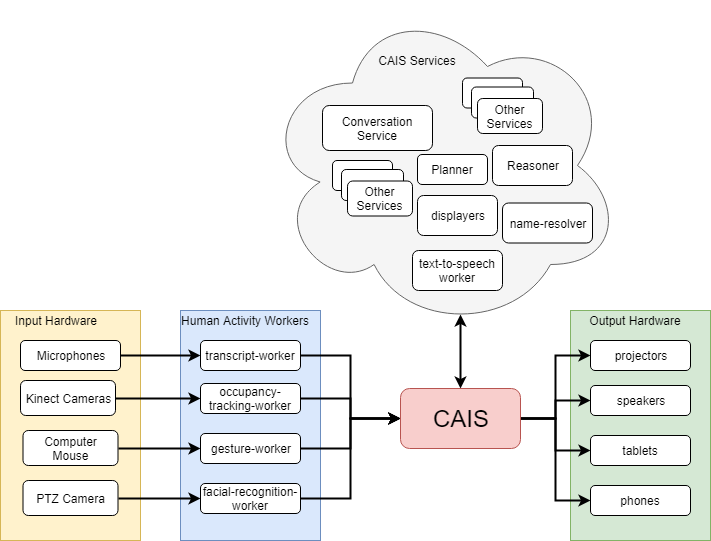
\includegraphics[width=0.5\columnwidth]{chapters/02_technology/figures/cais_high_level.png}
    \caption{High level diagram of CAIS architecture.}
    \label{fig:cais_high_level}
\end{figure}

As stated above, the architecture here is event-driven, such that workers can
be activated at any time, and then feeds through the CAIS, triggering further
modules as the event is fed forward. For example, the transcript-worker is
activated with the event of someone talking into the system. Important to
this model is the communication methods which we utilize within our system.
Principally, we utilize a distributed message queue wherein modules can
register as producers and consumers, allowing messages to be passed, which
act as the events of the system. One of the requirements here is that we
expect that multiple modules may consume from the same producer, allowing
a singular event to trigger multiple pieces downstream. Generally, each
``core'' module of the CAIS acts as both a producer and consumer, with
the exception of the edge modules, such that input modules (e.g. 
transcript-worker) are producers and the output modules (e.g. speaker-worker)
are consumers. For our purposes here, we utilize 
RabbitMQ~\cite{pivotal_software_rabbitmq_2020}, a commercially available
message broker that fits our needs. To accomplish the above message queue
requirement With RabbitMQ, we utilize a broadcast model where modules
subscribe to event topics, where each topic is made up of a number of pieces. 
Each topic is
unique to a given event, and that the topic pieces are specified in a manner of
least specific (e.g. the module name) to most specific (e.g. the event action).
Any number of consumers can subscribe to a given topic, each receiving the same
event. For example, the transcript-worker produces output on the topic
``transcript.result.interim'' (for in-progress speech transcription) and
``transcript.result.final'' (for finished speech transcription). Any number of
consumers could then listen to either of those channels, and be activated by
a transcription event. In rare cases, certain modules utilize RPC communication,
principally for modules that are hooked to a specific hardware device (e.g.
speaker-worker which is connected to a system's speakers). However, it's
expected that while communication to the module itself is done via a single RPC
queue, the module then broadcasts out events relating to what it is doing. For
the speaker-worker, this means that it will receive a sentence to output
via the speakers, and it will issue an event ``speaker.speak.begin'' before
it starts playing the sound, and ``speaker.speak.end'' when it finishes, which
any module can subscribe to.

Finally, for services that are not necessarily core to the CAIS itself, but
rather contain information or outside capabilities, we largely rely upon
utilizing standard TCP calls to these services. These services are, but not
limited to, things like databases, prover, external APIs.

A limitation of this approach is that each new link between modules introduces
additional latency to the system. However, within everything running on a high
speed connection, the added latency is roughly ~8ms per link. This throughout
is not largely felt by the user over the bottleneck of slower operations
involved with calling some of the external services and complex operations
of the CAIS, such as transcription service for parsing microphone input.

We are confident in our approach, and are in good company with  prior work that
followed a similar approach, such as the work done by
Brooks~\cite{brooks_intelligent_1997}. However, unlike this prior work, through
the use of RabbitMQ, the links between modules are that of topics, and not
necessarily hard coded agent links.


% 5. Modules
\section{Implemented CAIS Modules}

\input{chapters/02_technology/05_modules/01_intro.tex}

%  1. transcript-worker
\input{chapters/02_technology/05_modules/05_transcript-worker.tex}

%  2. conversation-worker
%  3. MUIFOLD
%  4. spatial-context-worker
%  5. Reagent
%  6. orchestrator
%  7. executor
%  8. display-worker
%  9. speaker-worker



% 3. MUIFOLD
\chapter{Generic Understanding of Displayed Content and Interactions}

\section{Reagent}\label{sec:reagent}

The \textit{Reagent} system allows us a way to hook into the content that is
shown within the Electron framework discussed in Section~\ref{sec:cais}. The
system is broken up into two components, a central server and then the clients.
The central server is used to handle communication from the clients and the
larger CAIS architecture, as well as store information coming from the clients
for reference. This information includes the type of semantic elements exist on
the page, as well as an event stack for recorded user interactions within any
webview. Communication between the server and the clients is handled by using
websockets which facilitates real-time communication of data. To handle requests
from the CAIS, the server implements a RESTful API. The client are inserted as a
transparent layer on top of any opened webview within the system.  This
transparent layer then sets up a connection back to the central server, and then
semantically parses the page using standard DOM traversal via JavaScript
to identify key HTML structures with which a user
might interact with (e.g. a table or a plot), and uses this information to bind
appropriate event handlers to listen for user interactions, as well as for any
changes to the page's content. More specifically,

\begin{enumerate}
    \item Electron pre-loads the \textit{Reagent} system on top of the webview, and injects a websocket connection allowing it to communicate with the open webview and receive JSON-formatted events into an event buffer.
    \item Electron emits a ``DOM Ready" event to signal that the page has finished loading, whereupon \textit{Reagent} scans the page to see if it can detect any major HTML elements it should parse and bind to (e.g. a table).
    \item \textit{Reagent} injects additional code specific to the detected HTML elements that binds event listeners to these elements as well as assigning each a UUID --- an approach that makes \textit{Reagent} readily extensible to new types of elements. (We have implemented domain-independent layers designed for general tables and for plot.ly plots, and allow for domain specific layers as well.)
    \item Next, \textit{Reagent} creates a MutationObserver\footnote{https://mzl.la/1exU78d} to watch for any changes to the page. If changes are detected, it performs any necessary re-injections and re-bindings to ensure that all relevant elements remain instrumented.
    \item Finally, \textit{Reagent} sets up a listener such that if the webview
    is closed, the client disconnects and the server is alerted.
\end{enumerate}

This sequence of events is illustrated within Figure~\ref{fig:reagent}. As an example, we discuss how the
Reagent system would bind to a HTML table and the sorts of queries it would allow for from the user. A perfect data table
is made up of some number of columns and rows where the first row, if marked with the ``th'' tag, should be viewed
as a header row with labels for the columns, and then all subsequent rows marked with the ``td``` tag as data. Reagent
scans the table, generating a list of the column names and some simple heuristics about the structure of the table. Next,
assuming that Reagent has never seen a table on this site before, it first takes all of the headers and attempts to
normalize them as appropriate for its datatype using NLTK and WordNet. Take for example, a column labelled ``won''
for a column with numeric information. Here, the system first casts the word to the present tense of the verb (``win''),
and then pluralizes on its noun form (``wins''), giving us a title more likely to be said by humans. From here, we then
use WordNet to find the variations of the word (on both its noun and verb forms) and add them as entities, if missing,
to Watson Assistant to be used for intent classification on future queries.
Finally, the system binds listeners for user interaction, which in the case of a simple table would be if a user clicks on
a cell in a table or leaves their mouse hovering over it for greater than a second. For any interaction, the client
communicates with the server, which saves a JSON object of the interaction which contains what webview it occurred in,
generated reagent UUID of the element, what row/column the cell was in, contents of the cell, and the type of interaction
it was (e.g. mouseover or click).

During the scan of HTML elements, the system is capable of taking advantage of
content added for accessibility reasons. For example, in
Fig.~\ref{fig:screenshot}, the column for ``appearances'' was labelled ``APP''.
\textit{Reagent} identifies tags that may indicate more human-friendly terms,
such as tooltips that reveal explanatory text when a user hovers over an
element, and uses approximate text matching to infer likely associations where
possible.
In cases where the system is unable to disambiguate the semantic information, it
solicits a definition from the user. For example, with the ESPN table, the
system would ask the user (via synthesized voice) to mouse over ``the column
labeled  \textit{A}'' and state what is the attribute. Upon hearing ``Assign
attribute \textit{assists} to this column", \textit{Reagent} stores the
mapping in a dictionary, whereupon it becomes available to any subsequently
accessed bound elements on the same webpage or host site.

\begin{figure}
\centering
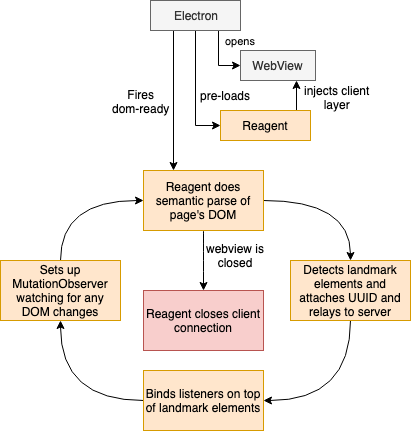
\includegraphics[width=0.45\textwidth]{figures/reagent.png}
\caption{Flowchart of the Reagent System.}
\label{fig:reagent}
\end{figure}

Through the transparent layer and central server described above, \textit{Reagent} enables
the executor to handle a wider range of queries that pertain to references
to the content within open webviews. At its most basic layer, the user can
query the system for the contents of the full table, what are the columns in a
table, as well as asking queries about statistics (e.g. max, min, or average)
of any given column. By capturing the interactions, it then allows the system
to handle queries that are for relative locations within the interacted with
element. For example, Figure~\ref{fig:screenshot} illustrates the state of the
display after the user has opened an ESPN football team roster webpage and
asked the system ``Show in a new table rows where \textit{appearances} are
greater than 35.''. Equivalently, the user might have asked ``Show in a new
table rows with this column greater than this.'' while pointing to a cell
under the column `APP' with the value of 35.\footnote{For a fuller set of
capabilities that includes query, sorting, and simple analytics like averaging,
a link to a demo video is available at \url{https://bit.ly/20GKvez}}.

\section{MUIFOLD}

MUIFOLD is a framework for building applications with interactions
between a large display and multiple concurrent mobile clients.
Before discussing the specifics of the architecture and
implementation, we first layout some overall design goals that
we had for our system.

\begin{enumerate}
    \item \textbf{Utilize web-based technologies.} As shown by
    the prior work, by exclusively using web-based technologies
    for the display and mobile clients, this greatly lowers the
    barrier of entry for users and as opposed to requiring custom
    native applications they must install. This also makes it easier
    to build new content given the overall ubiquity of the web.
    \item \textbf{Multi-User Support.} Our application should
    be able to support multiple mobile clients simultaneously.
    \item \textbf{Have low latency between interactions of client and display.} When a user performs some action on their client, the
    display server should reflect that change relatively quickly,
    aiming for under 70ms to prevent potential loss of precision
    in various tasks~\cite{ivkovic_quantifying_2015}.
    \item \textbf{Provide ability to handle generic web pages in
    addition to custom built pages.} In an ideal world, all
    content would be custom built for our framework, users may
    have existing web technology that they would like to use. We
    should provide a way to seamlessly, and without any changes from
    the third-party site developer, integrate that the site in a
    seamless fashion, even if with relatively basic interaction.
\end{enumerate}

\subsection{Architecture}

It is split into three modules, the display server, the
mobile client, and the application web-pages as shown in Figure \ref{fig:architecture_muifold},
specifics of which are detailed below. Communication between the
client and display server and then display server to web-pages is
done using WebSockets, which provide a full-duplex
communication channel over a single TCP connection. We utilize the
JavaScript Object Notation (JSON) format to transmit runtime
information. While this causes a slight increase on amount of bytes
sent over the wire compared to custom formats prior worked used,
this did not cause a noticeable degradation on performance and
latency as number of users scaled. Additionally, it is expected
that for custom client UIs that get opened, a WebSocket will
get opened that connects the client to a remote server hosting
the page they are interacting with, allowing for more
in-depth interaction.

\begin{figure}
\centering
  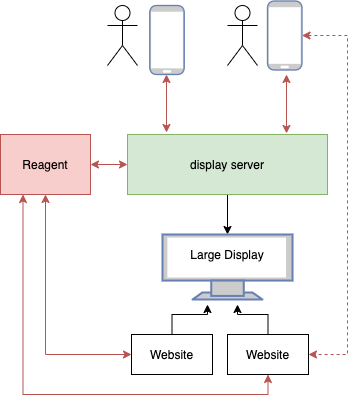
\includegraphics[width=0.8\columnwidth]{figures/muifold_architecture}
  \caption{Architecture of MUIFOLD. The red lines are WebSockets and the dotted line indicates an optional Web Socket depending on application needs.}
  \label{fig:architecture_muifold}
\end{figure}

\subsection{Display Server}

The display
server is based on our prior work on developing a virtual mouse
interface~\cite{peveler_virtual_2020}, which we quickly describe
here. The server runs an
Electron~\footnote{https://www.electronjs.org/} application, which
provides a chromium based engine to render web content. In the
display, the available screen real estate is divided into a grid,
and then websites are loaded into so-called ``webviews;; that then
takes up some amount of that grid. For example, in Figure
\ref{fig:display_server_grid}, we show a 4x4 grid with 3 open
webviews that take up differing amounts of the grid.

Manipulating the webviews, be it opening / closing them, moving them
around, or resizing them, is done through a REST API that accepts
a JSON object describing the type of change (e.g. open, close), an
ID of the webview if affecting an existing one, and
details on the change (e.g. change size to 2x2, move to 3x4 on grid).
When opening a webview, an additional parameter is accepted that
tells the system whether or not that component exposes a MUIFOLD
mobile UI, and a URL to the JavaScript files necessary to load and
run that UI. Requests to this API can come from the mobile UI or
from an external server unconnected to MUIFOLD. Communication
between the clients and display server happens via WebSockets where
client UIs pass information as to where their current cursor is
as well as potential actions to take (e.g. clicking or scrolling)
which the display server carries out on the webview underneath
the cursor (while leaving all other webviews alone). Through this
separation, clients are able to interact with different webviews
simultaneously if they so choose, or come together on one single
webview.

\begin{figure}
\centering
  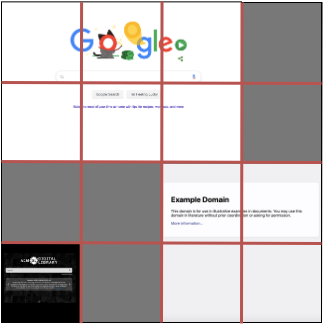
\includegraphics[width=0.65\columnwidth]{figures/display_server}
  \caption{Display Server grid with 3 open webviews where the red lines represent the grid that contains them.}
  \label{fig:display_server_grid}
\end{figure}

When opening webviews, the display server injects our
Reagent~\cite{peveler_reagent:_2019} service onto the page, which
first opens a WebSocket back to the display server. Reagent then
captures information about various semantic elements on the page,
and creates listeners for user interaction with that content. The
websocket provides a mechanism for the display server to
programmatically trigger actions like mouse clicks or sending
input specific to a given mobile device, while Reagent can report
back to the display service the specifics about an element being
interacted with, such as if the user clicks on a dropdown, Reagent
will report all available options for the dropdown. Finally,
Reagent sets up a monitor to re-bind itself in-case of content
changes on a page. By utilizing the programmatic interface,
we allow multiple users to concurrently be able to send events
and interact simulatenously on the same page as well as
on totally different open webpages. There is still a potential
for user collision (e.g. one user clicks on a link on a page or
scrolls a page while another user is doing something else), but this
is not a unique problem we face and is solved just through general
good manners by users.

\subsection{Mobile Client}

The web-based mobile client, like other frameworks, is presented to the enduser through a simple webpage that the user opens on their
mobile device. This
can be either through scanning a QR code displayed on the large
display, or by manually typing in the URL. The client is
written using the React JS
framework~\footnote{https://reactjs.org/}, which provides a
high-level interface for building interactive UIs in JavaScript.
React provides a declartive language for the UI to be built in,
and helps to redraw the DOM as necessary as parts of the underlying
application state changes. Additionally, React allows us to define
the pieces of our UI as components, which makes it easy for us to
re-use pieces of the generic UI a user is greeted with when opening
the client in custom webview specific UIs as they need (e.g. like
for enabling pointing).
Out of the box, the mobile client presents the user with a generic
UI capable of interacting with any content displayed by the
large scale display, shown in Figure ~\ref{fig:mobile_start_ui}. The principle interaction methods in this
interface are pointing, left clicking, and scrolling content, similar
to the common mouse most users are familiar with from traditional
desktop and laptop computers.

\begin{figure}
\centering
  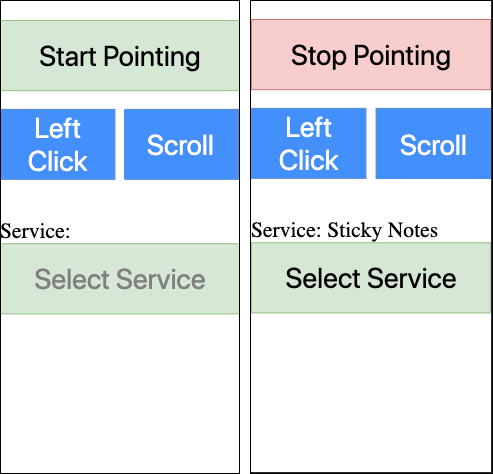
\includegraphics[width=0.65\columnwidth]{figures/generic_mobile_client}
  \caption{Generic Interface for mobile client. Left view shows
  screen while not currently pointing. Right view shows client
  while actively pointing and cursor is over a display that has a custom application UI.}
  \label{fig:mobile_start_ui}
\end{figure}

Pointing is done through relative raycasting, relying solely
on the phone's builtin gyroscope and accelerometer and no additional
hardware through the DeviceOrientation API. When a user initially
connects, a
cursor is shown for the user at the center of the screen. Then,
while pointing is activated, for each tick the sensors report
their current degree, this is compared against the last measured
degree, taking the difference. This is then run through a smoothing
function~\cite{casiez_1_2012} to eliminate effects of natural
jitter, both in the sensors themselves and from slight hand
tremors. The client then reports this degree change to the display
server which translates this into a x,y pixel translation,
moving the cursor appropriately. The client then receives
information from the display server on if the cursor now is atop
a service that implements its own application specific UI. A
limitation of this approach is that over time, the cursor
eventually suffers from drift between where the user is pointing
to and where the cursor actually is. Self correction for this
though is easy enough by turning off pointing, re-adjusting
pointing position, and then turning back on pointing that it
this is not a great enough hindrance to ruin the approach. One thing
we did worry about was that as a user moved around the room and
interacted with the screen at different distances and angles, the
ratio of
degrees to pixels would need to change as well. In practice however,
we found that keeping this constant did not have any negative
effect on usage, so long as users stayed within 5-10 meters from
the ``sweet spot''.

Left clicking on the mobile interface is similar to how might
expect left-clicking with a standard mouse on a webview. Clicks that
happen within input fields, however will create a modal to appear
on the mobile interface that can be used to update that input
field, allowing the user to update the form in a mobile friendly
way. For example, clicking on a dropdown would show all of
the available options, clicking on an input would open the
keyborad, etc. Finally, when a user points at a webview that
is marked as having its own mobile UI, the button at the bottom
of the generic UI will activate with the name of the webview
appearing above it, such as in the right image in Figure
\ref{fig:mobile_start_ui}.

When opening a webview specific UI, the client gets the
URL for the webview's JavaScript to power its mobile UI. This
is then loaded dynamically, and injected into the running
application and run. It's expected that the JavaScript file will
either hook into the existing React root webview specific UIs or
can use vanilla JavaScript to build the DOM and manage it that way.
However, as stated above, with React, developers can utilize
components of the generic UI into their design as makes sense,
such as making available a button to toggle on / off pointing. The
only requirements for these UIs is that they must implement a button
that returns the user to the generic UI, and that they do not
overwrite the React root for the generic UI. Figure
\ref{fig:application_specific_ui} gives an example of how such
a UI might work for a specific application, in this case one
to create sticky notes. This UI re-uses the pointer component,
though shifted to the bottom of the screen, with custom content
for creating sticky notes. Hitting the ``Canel'' button would
bring the user back to the generic UI.

\begin{figure}
\centering
  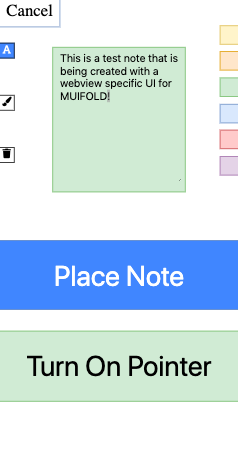
\includegraphics[width=0.40\columnwidth]{figures/application_specific_ui}
  \caption{Webview specific UI for a sticky notes application.}
  \label{fig:application_specific_ui}
\end{figure}



% 4. Formalizing the CAIS
\chapter{Formalizing the CAIS}

%    1. Deontic Cognitive Event Calculus
%        1. ShadowProver
%        2. Spectra
\section{The Cognitive Event Calculus}

To capture the room in a formal way, we employ the \textbf{deontic
cognitive event calculus} (\DCEC), a cognitive calculus and
intensional logic (Please see
the appendix for definitions of these terms).\footnote{We do not use the
  deontic components in \DCEC\ in this paper.}  While the full syntax
and inference schemata are outside the scope of this paper, we give a
brief overview.\footnote{For a more in-depth primer on the \DCEC, see
  the appendix in \cite{nsg_sb_dde_ijcai}.} \DCEC\ is a multi-sorted
quantified modal logic with a well-defined syntax and proof calculus.
\DCEC\ subsumes the event calculus~\cite{mueller_commonsense_2014}, a first-order
calculus used for modeling events and actions and their effects upon
the world.  The proof calculus of \DCEC\ is based on natural deduction
\cite{gentzen_investigations_1964} and includes all the introduction and elimination
rules for first-order logic, as well as inference schemata for the
modal operators and related structures.  \DCEC\ is a sorted system and
includes the built-in sorts shown in Table~\ref{syn:sorts}.

Table~\ref{syn:terms} presents the syntax of our language for forming
terms, while Table~\ref{syn:defs} presents a list of built-in function
symbols, which come from the standard event calculus, in our language.
Table~\ref{syn:formulae} shows the syntax for
formulae in the language, and finally Table~\ref{rules} shows a subset of
inference schemata needed for our current purpose. The main
inference schemata needed include $I_{\knows}$ and $I_{\believes}$,
which state that knowledge and belief are closed under the inference
system of $\DCEC$.  We also have inference schemata that let us go
from perception to knowledge ($I_1$), knowledge to belief ($I_2$),
common knowledge to knowledge ($I_3$), and from knowledge to
propositions that hold ($I_4$). Below, we also use \emph{derived
  inference schemata} for converting perceptions to knowledge,
knowledge to belief, common knowledge to belief,~labeled as
$D_{[\perceives \leadsto \knows]}$, $D_{[\knows \leadsto \believes]}$,
and $D_{[\common \leadsto \believes]}$ respectively
\cite{ArkoudasAndBringsjord2008Pricai}.


\begin{table}
\begin{footnotesize}
\begin{center}

\begin{tabular}{lp{8cm}}
\toprule
\textbf{Sort}    & \textbf{Description} \\
\midrule
\type{Agent} & Human and non-human actors.  \\

\type{Moment} &  Time points. E.g., $t_i$, $birthday(son(jack))$ etc. \\

  \type{Event} & Used for events in the domain. \\
  \type{ActionType} & Abstract actions
                      instantiated by agents.\\
  \type{Action} & Events that occur
                  as actions by agents \\
  \type{Fluent} & Representing states of the world.\\
  \type{Formula} & Represents any arbitrary formula\\
  \bottomrule
\end{tabular}
\caption{Basic sorts in the language}
\label{syn:sorts}
\end{center}
\end{footnotesize}
\end{table}




\begin{table}
\begin{footnotesize}
\begin{center}
  \begin{tabular}{lp{10.3cm}}
    \toprule
    \textbf{Terms} & \textbf{Explanation}  \\
    \midrule
    $x: S$ & A variable $x$ of sort $S$. E.g. ${a_i}:\type{Agent}$ representing
             an agent. \\
    $c: S$ & A constant $c$ of sort $S$. E.g. ${jack}:\type{Agent}$ representing
             an agent named ``jack.'' \\
$ f(t_1,\ldots,t_n)$ & A function expression. E.g. $\action(eating, john) $\\
    \bottomrule
  \end{tabular}
\caption{Syntax for terms in the language}
\label{syn:terms}
\end{center}
\end{footnotesize}
\end{table}

%% Moved the the tables for syntax, formula, and schema into the middle of
%% the reasoner-planner section
%% to force latex to put them onto the same page and save some space // Matt

To handle reasoning within \DCEC\, we utilize a quantified modal logic
theorem prover, \textsf{ShadowProver}, first presented in
\cite{nsg_sb_dde_ijcai,uncertaintyized_cognitive_calculus}.\footnote{The
  prover is available in both Java and Common Lisp and can be obtained
  at: \url{https://github.com/naveensundarg/prover}. The underlying
  first-order prover is SNARK, available at:
  \url{http://www.ai.sri.com/~stickel/snark.html}.}  The prover works
by utilizing a technique called \textbf{shadowing} to achieve speed
without sacrificing consistency in the system.  Shadowing is a
syntactic operation that converts any modal formula (or a set of
formulae) $\phi$ to a non-modal formula $\mathsf{shadow}[\phi]$ by replacing atomic
modal sub-formuale with propositional atoms.

\begin{table}
\begin{footnotesize}
\begin{center}
\begin{tabular}{lp{10.3cm}}
\toprule
\textbf{Function Symbols} $f$& \textbf{Sort}  \\
\midrule
$\action$ & $\Agent \times \ActionType \rightarrow \Action$\\
$ \initially$ & $\Fluent \rightarrow \Boolean$\\
  $\holds$ & $ \Fluent \times \Moment \rightarrow \Boolean $\\
  $ \happens$ & $ \Event \times \Moment \rightarrow \Boolean$ \\
  $ \clipped$ & $ \Moment \times \Fluent \times \Moment \rightarrow \Boolean$ \\
  $ \initiates$ & $ \Event \times \Fluent \times \Moment \rightarrow \Boolean$\\
  $ \terminates$ & $ \Event \times \Fluent \times \Moment \rightarrow \Boolean$ \\
  $ \prior$ & $\Moment \times \Moment \rightarrow \Boolean$\\
\bottomrule
\end{tabular}
\caption{Builtin function symbols in the language}
\label{syn:defs}
\end{center}
\end{footnotesize}
\end{table}


\begin{table}
\begin{footnotesize}
\begin{center}
\begin{tabular}{lp{10.3cm}}
\toprule
\textbf{Formula Expressions} $\phi$& \textbf{Explanation}  \\
\midrule
$A(\ldots)$ & Atomic formulae such as $\holds(raining, t_2)$\\
$\neg \phi$ & Negations. E.g., $\lnot\holds(raining, t_2)$\\
$\phi \lor \psi$ & Disjunctions. E.g., $\holds(cloudy, t_2)
\lor \holds(sunny, t_2)$\\
$\phi \lif \psi$ & Implications. E.g.,  $\holds(cloudy, t_2) \lif
                   \lnot \holds(sunny, t_2)$\\
$\perceives (a,t,\phi)$ & Agent $a$ perceives at time $t$ that $\phi$
                          occurs or holds \\
$\knows (a,t,\phi)$ & Agent $a$ knows at time $t$ that $\phi$
                          occurs or holds \\
$\believes (a,t,\phi)$ & Agent $a$ believes at time $t$ that $\phi$
                          \\
$\intends (a,t,\phi)$ & Agent $a$ intends at time $t$ that $\phi$
                          \\
$\desires (a,t,\phi)$ & Agent $a$ desires at time $t$ that $\phi$
                          \\

$\says (a,b,t,\phi)$ & Agent $a$ communicates to agent $b$ at time $t$
                       that $\phi$ \\
$\common (t,\phi)$ &At time $t$ $\phi$ is common knowledge.
                          \\
\bottomrule
\end{tabular}
\caption{Syntax for formulae in the language}
\label{syn:formulae}
\end{center}
\end{footnotesize}
\end{table}





{ % begin box to localize effect of arraystretch change
\renewcommand{\arraystretch}{2}

\begin{table}
\begin{footnotesize}
\begin{center}
  \begin{tabular}{lp{8cm}}
\toprule
\textbf{Inference Scheme} $\phi$& \textbf{Explanation}  \\
\midrule
$\infer[{[I_{\knows}]}]{\knows(a,t_2,\phi)}{\knows(a,t_1,\Gamma), \
    \ \Gamma\vdash\phi, \ \ t_1 \leq t_2}$ & From prior knowledge, agents
                                             can infer new knowledge
                                             at at later time.\\
$\infer[{[I_{\believes}]}]{\believes(a,t_2,\phi)}{\believes(a,t_1,\Gamma), \
    \ \Gamma\vdash\phi, \ \ t_1 \leq t_2} $ & From prior belief, agents
                                              can infer new beliefs at
                                              a later time.\\
$\infer[{[I_1]}]{\common(t,\perceives(a,t,\phi)
   \lif\knows(a,t,\phi))}{}$ & It is common knowledge that perception
                               leads to knowledge\\
$\infer[{[I_2]}]{\common(t,\knows(a,t,\phi)
    \lif\believes(a,t,\phi))}{}$ & It is common knowledge that
                                   knowledge leads to belief \\
$\infer[{[I_3]}]{\knows(a_1, t_1, \ldots
    \knows(a_n,t_n,\phi)\ldots)}{\common(t,\phi) \ t\leq t_1 \ldots t\leq
    t_n}$ & Definition of common knowledge \\
$\infer[{[I_4]}]{\phi}{\knows(a,t,\phi)}$ & If $\phi$ is known, then
                                            $\phi$ holds\\
\bottomrule
\end{tabular}
\caption{Inference schema}
\label{rules}
\end{center}
\end{footnotesize}
\end{table}
}

The prover can be equipped
with multiple sets of inference schemes $\rho^p_{q}$, where
$q\in\mathbb{N}$ denotes the degree of the schemes (e.g. $0$ for
propositional schemes, $1$ for first-order quantifier schemes, etc.)
and $p\in\{0,1\}$ denotes the modality of the schemes. For example, pure
propositional logic and first-order schemes are given by $\rho^0_{0}$
and $\rho^0_{1}$, while modal
propositional or modal first-order schemas are given by $\rho^1_{0}$ and
$\rho^1_{1}$.


% Given any arbitrary formula $\phi$, $\mathsf{A}_{[\phi]}$ is a unique
% atomic (propositional) symbol. We define the \textsf{level} of a
% formula: $\mathsf{level}(\phi) = 0$ if $\phi$ is purely propositional;
% $\mathsf{level} (\phi) = 1$ if $\phi$ is purely first-order; and
% $\mathsf{level} (\phi) = 2$ if $\phi$ is modal.  Given the above
% definition, we can define the operation of \textbf{shadowing} a
% formula to a level.  To shadow a formula $\chi$ to a level $l$,
% replace all subformulae $\chi'$ in $\chi$ such that
% $\mathsf{level}(\chi')>l$ with $\mathsf{A}_{[\chi']}$
% simultaneously. We denote this by $\mathsf{S}[\phi,l]$.
Starting from a set of modal formula $\Gamma$ as premises and a goal
$\phi$, the prover operates in two phases. In the first phase, it
expands $\Gamma$ using the modal schemes $\rho^1_{0}$ and
$\rho^1_{1}, $ and checks if $\phi$ is contained in the expanded
set. In the second phase, the prover applies the non-modal schemes
$\rho^0_{0} $ and $\rho^0_{1}$ to $\mathsf{shadow}[\Gamma]$ and checks whether
the expanded set contains $\mathsf{shadow}[\phi]$. The two phases are repeated
till either the goal is reached or no expansions happen.

Planning for the room is handled by \textsf{Spectra}, a planner based
on an \emph{extension} of the STRIPS-style
planning language, and backed by \textsf{ShadowProver}. In this planning formalism, arbitrary
formulae of \DCEC\ are allowed in states, actions, and goals.  For
instance, valid states and goals can include: \emph{``No three blocks
on the table should be of the same color.''}  and \emph{``Jack
believes that Jill believes there is one block on the table.''}

\begin{comment}
\subsection{Non-modal Systems are not Enough}
\label{sect:prop_not_enough}
 In an \textbf{extensional} system, two
terms $t_1$ and $t_2$ are considered to be identical if they denote
the same set of objects. Logics such as propositional logic,
first-order logic, higher-order logic, etc. are extensional systems
and are best suited to modeling states of the world. In an
\textbf{intensional} system, the meaning of a term $t$ is dependent on
the context $C$ in which it occurs. Modal logics are intensional
systems. \DCEC\ is an {intensional} logic in the sense that it has
intensional operators.\footnote{Please note that there is a vast difference between
  intension and intention.} Intensional systems are crucial for modeling
theory-of-mind reasoning.

For example, using an extensional system such as first-order logic to
model theory-of-mind reasoning leads to unsound inferences as shown
below, in which we have an agent $r$ that knows the manager of a team
is the most responsible person in the team.  Agent $r$ does not know
that $\mathit{Moe}$ is the manager of the team, but it's true that
$\mathit{Moe}$ is the manager.  If the knowledge operator $\mathbf{K}$
is a simple first-order predicate, we get the proof shown below, which
produces a contradiction (that $r$ knows that $\mathit{Moe}$ is the
manager) from true premises.  This unsoundness persists even with more
robust representation schemes in extensional logics
\cite{selmer_naveen_metaphil_web_intelligence}.

\vspace{10pt}

\begin{minipage}[b]{0.7\textwidth}
\begin{footnotesize}
 \begin{footnotesize}
\begin{equation*}
\begin{aligned}
&\fbox{1}\ \ \mathbf{K}\left(r,\
  \mathsf{Manager}\left(\mathit{team}, \mathit{mostResponsible}\left(\mathit{team}\right) \right)\right) \mbox{
  {\color{gray}; given}} \\
&\fbox{2}\ \ \lnot \mathbf{K}\left(r,\mathsf{Manager}\left(\mathit{team}, \mathit{Moe}\right)\right) \mbox{
  {\color{gray}; given}}\\
&\fbox{3}\ \ \mathit{Moe} = \mathit{mostResponsible}\left(\mathit{team}\right)  \mbox{
  {\color{gray}; given}}\\
&\fbox{4}\ \ \mathbf{K}\left(r,\mathsf{Manager}\left(\mathit{team}, \mathit{Moe}\right)\right)  \mbox{
  {\color{gray}; first-order inference from \fbox{3} and \fbox{1}}}\\
& \fbox{5}\ \ \mathbf{\bot}  \mbox{
  {\color{gray}; first-order inference from \fbox{4} and \fbox{2}}}
\end{aligned}
\end{equation*}
\end{footnotesize}
\end{footnotesize}
\end{minipage}
\end{comment}


%    2. Formalization of Requirements

%    3. Formalization of Modules into DCEC

%    4. Properties of a CAIS (e.g. inRoom)


% 5. Use Cases
\chapter{Grounding Use-Cases of our CAIS}\label{chap:use_cases}

In this section, we introduce two use-cases for our CAIS to help demonstrate
its capabilities in the realm of planning and plan recognition. For each
use case, we first present it in plain, informal discussion, and follow it
with a formalization within the CEC.

%    1. Cognitive Blockworld
\subsection{Overview}

We now introduce the \emph{cognitive-polysolid framework} (CPF), a
class of problems that we use for our experiments. In these problems,
both human agents and polysolids are represented and questions concern the
cognitive states of the humans. For our purposes,
we classify our polysolids as regular 3D shapes, such as cubes, cylinders, spheres, etc.
that do not contain any holes or gaps in them. Using
the framework, we can generate a \emph{cognitive-polysolid world
instantiation}, where an instantiation has some number of polysolids,
declares how they can be moved, and specifies any agents and their possible
beliefs or knowledge about the polysolids and other agents.

CPF subsumes the familiar ``blocks world,'' described for instance in
\cite{nilsson_principles_1982}, which has long been used for reasoning and
planning tasks.  The framework gives us both a physical and cognitive
domain unlike the purely physical blocks world domain (The formal
logic used in \cite{nilsson_principles_1982} is purely extensional, as it is
simply first-order logic).  Since the physical complexities of blocks
world problems have been well explored
\cite{gupta_complexity_1992,slaney_blocks_2001}, we emphasize the cognitive extensions
of it.

The cognitive-polysolid world instantiation we focus on contains some finite number
of cubes/blocks and a table large enough to hold all of them.  Each block is
\texttt{on} one other object; where that object can be another block or the
table.  A block is said to be \texttt{clear} if there is no block that
is on top of it.  To move the blocks, an agent can either
\texttt{stack} (placing a block on the table on top of another block)
or \texttt{unstack} (taking a block that is on top of another block
and placing it on the table).  Before stacking a block onto another, both need
to be clear; when unstacking, the top block must be clear beforehand.
After stacking the blocks, the bottom block is then not clear, and
after unstacking, it is then now clear.


%    2. Sticky Notes
\section{Sticky Notes}

In this section we present our digital sticky notes use-case and application. This application provides
a more real-world usage of our technologies versus the more abstract Cognitive Block World, though is
still simple enough to be readily understandable. This use-case was designed to be as analogous to the
traditional pen-and-paper design as possible, aiming just to replace the interfaces with digital equivalents
while retaining the usage model. First, there is a shared global screen, on which the digital notes can be placed
or removed. This screen is large enough to accommodate several users standing in front of it at the same time,
and that the notes that are displayed on the wall are large enough to be read from a few feet away. To interact
with the wall, each user utilizes their cellphones to go to a specific URL in their browser. This webpage
asks for their name, and then they are free to begin. On their phone, a user is
first presented with buttons to create a new note and to pick a note up off the global screen. On hitting the
create note button, they are greeted with an interface to allow them to create a note, choose its color, etc.
Once they are satisfied with the content, they can click the button at the bottom of the UI to place the note.
This then opens their camera on their phone, showing the contents now on the screen, and the user then points
their camera to the part of the display they wish to place their note, clicking with their finger on their screen.

\begin{figure}
    \centering
    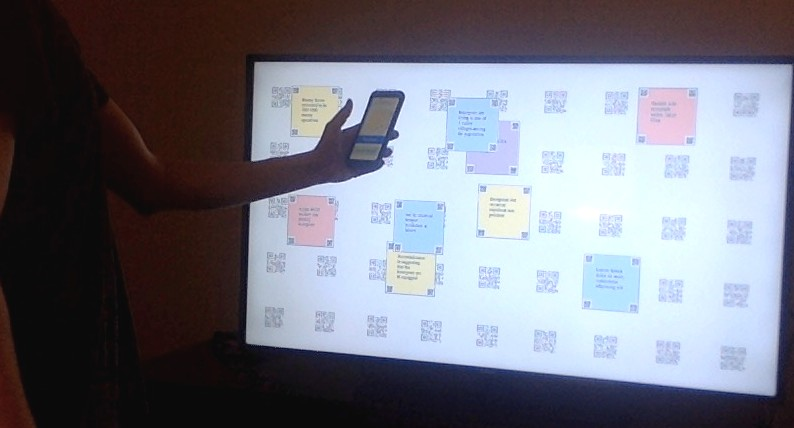
\includegraphics[width=0.45\textwidth]{figures/person_using}
    \caption{Someone using the sticky note application with their phone.}
      ~\label{fig:someone_using}
\end{figure}



% 6. Planning and Plan Recognition
\chapter{REASONING, PLANNING, AND PLAN RECOGNITION IN CAIS}\label{chap:planning}

%    1. Introduction
\section{Introduction}

Within these cognitive and immersive systems, it remains paramount that
our overseeing AI is capable of providing assistance to the participating
agents. As agents operate in the room, they are usually operating in pursuit
of a goal, committing actions to get them closer to accomplishing it. For
the over-seeing agent to increase in power, the system must be able to help
the user along their plans. To accomplish this, the system utilizes ``plan
recognition'', wherein given partial observations of actions, and knowledge
of possible goals, it infers the plans of its agents.


%    2. Prior Work
\section{Prior Work}

Planning, and more specifically plan recognition, is a rich field of
research that has a broad range of prior work that we draw from. For planning,
one branch of work is ``deductive planning'', wherein given a goal and a series 
of axioms,
the resulting proof gives a plan structure~\cite{green_application_1969}. This
approach is attractive as it allows the usage of first-order logic to define
our world, and the state transitions. Further work was done to handle concepts
of conditional branching, plan composition, and 
recursion~\cite{metzing_plan_1989,biundo_deductive_1992,rosenschein_plan_1981}.
However, through the regular use of FOL, we see a larger potential of ending
up with side-effects of actions, which can be undesirable for planning. An
alternative concept is through the usage of STRIPS-style 
planners~\cite{fikes_strips_1971}. Within these planners, each action is
defined via a complete structure with pre-conditions and post-conditions for
each action. This approach is attractive as it provides a useful mechanism for
dealing with the framing problem~\cite{mccarthy_philosophical_1969}. However,
these planners generally utilize a predicate calculus that lacks the full
expressiveness of first-order logic, not to mention higher order logics like
the \CEC. While STRIPS-styles planners work well across many domains, they
rely on deterministic planning. Extending the concept, conditional nonlinear
planners~\cite{peot_conditional_1992} and partial 
planners~\cite{pryor_planning_1996}
provide a mechanism for dealing with non-deterministic plans through if-else
like structures. However, this comes at a cost of increased complexity and
combinatorial explosion of states without ensuring some limitation on the
expressivity~\cite{rintanen_constructing_1999}. Given that we aim for increased 
expressivity, we do not consider these approaches herein. As such, we also do
not concern ourselves with other extensions to classical planners such as 
probabilistic 
planners~\cite{boutilier_decision-theoretic_1999,kaelbling_planning_1998}.

Independent of the specific formalisms and technology
that we bring to bear, we need to
model the mental states of humans in order to engineer AI
systems that understand and interact well with them.
For example, work in human-robot teaming has focused on
the use of planning techniques that take human goals and
mental states into account~\cite{briggs_multi-modal_2012}.
In addition, work on human-aware task planning for mobile robots
\cite{cirillo_human-aware_2009} has used \emph{predicted} plans of humans to
guide the system's own planning.
\cite{talamadupula_coordination_2014,chakraborti_planning_2015} showed this
approach more explicitly, representing and reasoning over a subset
of the humans' mental states relevant to the autonomous system's planning
problems.
Recent work has adapted these ideas to proactive decision making
\cite{sengupta_radar_2017,kim_towards_2017} and smart-room environments
\cite{chakraborti_mr._2017}.  \cite{pearce_etal_social_planning_aaai2014}
note the importance of what they call ``social planning,'' which
includes an agent achieving a goal via the modification of the mental
states of others.\footnote{Our example here is briefly returned
to later in ``Prior/Related Work and Novelty.''}

While these papers confirm the importance of formalizing and reasoning
about mental states within the planning process, they seem to us to lack the formal and
computational machinery needed to mechanize a full human-level theory
of mind --- let alone such a theory of mind \emph{and} the
requirements of a CAIS that we set out below.\footnote{Note that in
  the present paper there is a limit to the theory-of-mind-modeling
  ``power'' we insist an overseeing AI have.  E.g., we don't require
  that an AI overseeing an environment populated with humans have
  so-called \textit{phenomenal consciousness}, a form of ``what's it's
  like to'' consciousness characterized by \cite{bbs.block}, and
  claimed by \cite{sb_billion_conscious_robot}, to be impossible for a
  mere machine to possess.  In sharp contrast with phenomenal
  consciousness, \textit{cognitive consciousness} consists only in the
  logico-mathematical \emph{structure} of human-level (and, indeed,
  above) cognition, instantiated through time.  While cognitive
  consciousness can be characterized axiomatically with help from the
  formal languages we introduce below for cognitive calculi
  \cite{axiomatizing_consciousness1}, in the present paper we do not
  require the AI overseeing a CAIS have even cognitive consciousness,
  and we specifically do not require, at this early point in our work
  on cognitive-and-immersive systems, cognitive
  \emph{self}-consciousness, despite the fact that the latter is
  something that has been significantly mechanized and implemented
  \cite{roman2015_robot_self-con,sb_on_knowledge_game}.}  We now turn
to the presentation of the requisite formal and computational
machinery.

%    3. Defining Planning
\section{Defining Planning and Plan Recognition}

Before continuing, we explicitly define here the components of planning. We base our
work off of the definitions by Ramírez and Geffner~\cite{ramirez_plan_2009}.
Within this work, we utilize the STRIPS planning problem formalism, where each problem is the
tuple $P = \langle F, I, A, G \rangle$. For this tuple, $F$ stands for the set of
fluents that can define the state of world, $I \subseteq F$ is the initial state of
fluents, $G \subseteq F$ is the goal state of fluents, and $A$ is the set of actions
available to an agent. For each action $a \subseteq A$, it has a list
of preconditions, and then a list of post conditions to change the current
state of the world. An example definition of an action from the blocksworld domain is shown
in Listing~\ref{lst:strips}. Completion of a planning problem is then the computation of
an action sequence, $\pi = a_{1}, a_{2}, ..., a_{m}$, where each
$a_{i} \subseteq A$, and that following the action sequence starting at $I$
will arrive at $G$.

\begin{lstlisting}[caption=Stack action defined in STRIPS style,label={lst:strips}]
    (define-action stack [?x ?y]
        {
            :preconditions [
                (On ?x Table)
                (Clear ?x)
                (Clear ?y)
            ]
            :additions     [(On ?x ?y)]
            :deletions     [
                (Clear ?y)
                (On ?x Table)
            ]
        }
    )
\end{lstlisting}

As stated above, plan recognition on the other hand is planning in reverse,
wherein we now have only observations of agents to compare against a given plan.
Any computed $\pi$, be it from a plan library or constructed on the fly, then
must satisfy a given observation sequence.

From this, we can more regularly define the plan recognition problem. A plan recognition
problem can be defined as the tuple $R = \langle P, \mathcal{G}, O \rangle$, where
$P = \langle F, I, A \rangle$ as the planning domain (using the above terms),
$\mathcal{G}$ is the set of possible goals $G \subseteq F$ and
$O = o_{1}, o_{2}, ...., o_{n}$ is the observation sequence by agents where each
$o_{i}$ being an action in $A$. The observation sequence is then a subset
of a given action sequence wherein each observation matches into the action
sequence, where they follow the same ordering, but that there may be some missing
actions. For example, for the given action sequence $\pi = {a,b,c,d,e}$, then
the sequences ${a,c,e}$ and ${b,d,e}$ are valid, while ${c,a,e}$ is not.


\section{Automated Reasoner and Planner}\label{sec:automated_reasoner_planner}

\subsection{ShadowProver}

To allow our CAIS utilize the reasoning as defined in 
chapter~\ref{chap:formalizing}, we employ an automated theorem prover,
\textsf{ShadowProver}~\cite{govindarajulu_shadowprover_2018}\footnote{The
  prover is available in both Java and Common Lisp and can be obtained
  at: \url{https://github.com/naveensundarg/prover}. The underlying
  first-order prover is SNARK, available at:
  \url{http://www.ai.sri.com/~stickel/snark.html}.}. Traditionally,
first-order modal logic theorem provers
that can work with arbitrary inference schemata are built upon first-order
theorem provers. They achieve the reduction to first-order logic via two
methods. In the first method, modal operators are simply represented by
first-order predicates as in the example shown above. This approach is the
fastest but can quickly lead to well-known inconsistencies as demonstrated.
In the second method, the entire proof theory is implemented intricately in 
first-order logic, and the reasoning is carried out within first-order
logic. Here, the first-order theorem prover simply functions as a
general-purpose declarative programming system. This approach, while
accurate, can be excruciatingly slow.

\textsf{ShadowProver} utilizes a different approach to the above to achieve
speed without sacrificing consistency in the system. At the core of this
approach is a technique named ``shadowing'', wherein ShadowProver applies a
syntactic operation to convert any modal formula (or a set of formulae) $\phi$
to a non-modal formula $\mathsf{shadow}[\phi]$ by replacing the atomic modal
sub-formulae with propositional atoms. Through tis, ShadowProver is then able
to alternate between applying the high-level modal inference schemata and calling
out to a dedicated first order prover, until a proof has been found or not for the
given axioms and goal statement.

\subsection{Spectra}

Planning for our CAIS is handled by \textsf{Spectra}~\cite{govindarajulu_spectra_2018},
and planner based on an \emph{extension} of the STRIPS-style planning language discussed
above. At the core of \textsf{Spectra} is a backing of \textsf{ShadowProver} for resolving
actions. Through this, we can extend our planning formalism in several important
ways, namely that we allow arbitrary formulae of the \CEC\ in the definition
of states, actions, and goals. For instance, valid states and goals can
include: \emph{``No three blocks on the table should be of the same
color.''}  and \emph{``Jack believes that Jill believes there is one block on
the table.''}.

\section{Solving False-Belief Task in CAIS}\label{sect:false_belief}

\begin{figure}
\centering
  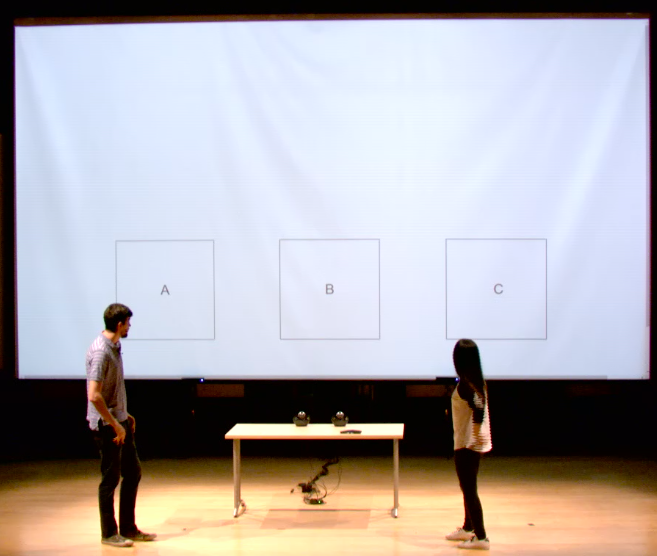
\includegraphics[width=0.7\columnwidth]{chapters/06_planning/figures/blockworld_demo_start.png}
  \caption{Starting state of our system.}
  \label{fig:blockworld_start}
\end{figure}

As a demonstration of our formalization process, we utilize our CAIS to solve the
false-belief task from before, modified to fit our CAIS. To accomplish this,
we instantiate a very elementary blocks world that involves only three blocks
named $\ablock$, $\bblock$, and $\cblock$, which all start on the
table. This is represented in the $\CEC$ as:

\begin{center}
\begin{tabular}{ c c }
    \holds(\on(\ablock, \ctable), 0) & 
    \holds(\clear(\ablock), 0)\\
    \holds(\on(\bblock, \ctable), 0) &     
    \holds(\clear(\bblock), 0)\\
    \holds(\on(\cblock, \ctable), 0) & 
    \holds(\clear(\cblock), 0)
\end{tabular}
\end{center}

In this instantiation, there are then two participants, \humana\ and \humanb\,
and then the block world is shown on the center screen in front of them. This
is shown in Figure~\ref{fig:blockworld_start}. We now provide below a sequence
of events that our agents act upon, providing the formalization of each action
into the \CEC\ as well as the fluent changes at each step of the time. If the
fluent is not removed by a step, then we assume that it carries over from the
previous step as is.

\begin{center}
\begin{tabular}{l | l | l}
    $t$ & Event in Natural Language & Event in \CEC\ \\
    \hline
    1 & \humana\ enters and registers with the CAIS & \happens(\register(\humana), 1) \\
    2 & \humanb\ enters and registers with the CAIS & \happens(\register(\humanb), 2) \\
    3 & \humana\ stacks block \ablock\ onto block \bblock\ & \happens(\stack(\ablock, \bblock), 3) \\
    4 & \humanb\ deregisters and leaves the CAIS & \happens(\deregister(\humanb), 4) \\
    5 & \humana\ unstacks block \ablock\ from block \bblock\ & \happens(\unstack(\ablock, \bblock), 5)
\end{tabular}\label{table:false_belief_actions}
\end{center}

\begin{center}
\begin{tabular}{l | l | l}
    $t$ & Added Fluent & Removed Fluents \\
    \hline
    1 & \holds(\inCAIS(\humana), 1) & \\
    2 & \holds(\inCAIS(\humanb), 2) & \\
    3 & \holds(\on(\ablock, \bblock)), 3) & \makecell[l]{
        \holds(\on(\ablock, \ctable), 2) \\
        \holds(\clear(\bblock), 2) \\
    }\\
    4 & & \holds(\inCAIS(\humanb), 3) \\
    5 & \makecell[l]{
        \holds(\on(\ablock, \ctable), 5) \\
        \holds(\clear(\bblock), 5) \\
    } & \makecell[l]{
        \holds(\on(\ablock, \bblock), 4) \\
    }
\end{tabular}\label{table:false_belief_fluents}
\end{center}

For this test, we utilize our weakest form of vicinity for agents, wherein
all events and fluents that happen within the room are in the vicinity of
any agent in the CAIS, and as such the agent can perceive them. If an agent
is outside the CAIS, then they are considered outside the vicinity of those
events and fluents, and will thus not perceive them. Additionally, for
any agents in the CAIS, they know, per our definition of $\textbf{I}_{1}^{f}$
that then all agents, being in the CAIS not only perceive the fluents for
themselves, but also that they perceive the other agents perceiving those
fluents as well. Additionally, we know from $\textbf{I}_{3}^{f}$ that our
CAIS also perceives all fluent changes, and perceives the agent perceiving
these fluents as well. From instantiations of $R_{1}$ - $R_{4}$ of the \CEC\
inference schemata, we can derive from these perceptions the state of beliefs
of our agents at any given time step to match the fluents that they perceive
at that time step.

\begin{figure}
  \begin{center}
    \begin{minipage}[b]{0.25\textwidth}
      \begin{flushleft}   
        \begin{footnotesize} \underline{\humana's beliefs}\\
          \vspace{4pt}
          \vspace{-4pt}
          \textbf{belief}:
        \end{footnotesize}
      \end{flushleft}    
      \begin{center} \begin{tikzpicture}[auto centering, background rectangle/.style={fill=white}, show background rectangle]
          \node[style=block] (C) {$C$};
          \node[style=empty] (E) [above=of C] {};
          \node[style=block] (B) [left=of C, left=.5cm of C] {$B$};
          \node[style=block] (A) [left=of B, left =.5 cm of B] {$A$};
        \end{tikzpicture}
      \end{center}
    \end{minipage}
   \hspace{50pt}
    \begin{minipage}[b]{0.25\textwidth}
      \begin{flushleft} 
        \begin{footnotesize} \underline{\humanb's  beliefs}\\                          
          \vspace{4pt}
          \vspace{-4pt}
          \textbf{belief}:
        \end{footnotesize}
      \end{flushleft}   \begin{tikzpicture}[auto centering, background rectangle/.style={fill=gray!25}, show background rectangle]
        \node[style=block] (B) {$B$};
        \node[style=emptyA] (E) [above=of C] {};
        \node[style=block] (A) [above=of B] {$A$};
        \node[style=block] (C) [right=of B, right=.5cm of B] {$C$};
        \node[style=empty] (F) [right=of C] {};
      \end{tikzpicture}
    \end{minipage}
  \end{center}
  \caption{Depiction of agents' mental states with the shaded portion indicating that \humanb\ is not in the room.}
  \label{fig:mom-example}
\end{figure}
 
We now move onto solving the false-belief task for our CAIS, and we consider
the world now after the completion of step 5. At this point, we wish to see
where the CAIS believes
the blocks are, as well as where it believes that \humana\ and
\humanb\ think the blocks are, focusing primarily on block A.  We ask
our overseeing AI three questions, translating them into the \CEC:

\begin{center}
\begin{tabular}{l|l}
    Where does the CAIS believe block \ablock\ is? & $\exists x (\believes(CAIS, 5, \holds(\on(\ablock, x), 5)))$ \\
    \makecell[l]{Where does the CAIS believe \\ \hspace{1cm}\humana believe block \ablock\ is?} & $\exists x (\believes(CAIS, 5, \believes(\humana, 5, \holds(\on(\ablock, x), 5))))$ \\
    \makecell[l]{Where does the CAIS believe \\ \hspace{1cm}\humanb believe block \ablock\ is?} & $\exists x (\believes(CAIS, 5, \believes(\humanb, 5, \holds(\on(\ablock, x), 5))))$
\end{tabular}
\end{center}

\noindent
For the first two questions, the CAIS and the \humana\ perceived all fluent
changes within the room, and so the answer should be the same, that block \ablock\ 
is on the table. For the third question, as \humanb\ has left our room, and thus
did not perceive the \unstack\ action, should still believe that the \ablock\
is on \bblock\. This state of affairs is captured in Figure~\ref{fig:mom-example}.
Through \textsf{ShadowProver}, we obtain an answer to the above question
of where each agent believes the block is: 

\begin{center}
\begin{tabular}{l}
     $\believes(CAIS, 5, \holds(\on(\ablock, \ctable), 5))$\\
     $\believes(CAIS, 5, \believes(\humana, 5, \holds(\on(\ablock, \ctable), 5)))$ \\
     $\believes(CAIS, 5, \believes(\humanb, 5, \holds(\on(\ablock, \bblock), 5)))$
\end{tabular}
\end{center}

From this, we have now shown that our CAIS possesses  ``theory of mind'', able to
track beliefs of both itself and contained agents, and moreover answer questions
about it. This provides a valuable baseline of ability to our system as we move
onto planning and plan recognition.

%    3. Single-Step Planning for Intent Resolution

\section{Intent Resolution}

We now move onto utilizing elements of planning, from which we deal with
the problem of intent resolution within our CAIS.
Ideally, any action carried out by our humans within the room would be as explicit
as possible. Indeed, when using something like MUIFOLD, this explicitness is handled for
the user under the hood by the app, tying together what note or block they're interacting
with, and what action they're attempting to accomplish with it. However, through voice,
providing the full explicit action may be difficult or 
impossible~\cite{kephart_embodied_2019}. To demonstrate this
behavior in more exact terms, we provide a motivating example. Imagine that within a CAIS, there
are two agents working with the sticky notes domain. Similar to work shown by
Bolt~\cite{bolt_put-that-there:_1980} a user may point to a note and say "Delete that
note". Alternatively, for reference a note by color on the screen, a user may say "Delete the blue
note". In both cases, while our system provides us with a ``\delete'' intent, we are not
provided an exact note we wish to operate on, and the system has to determine it from
context. We now talk through our algorithm for resolving the intent into something that
is actionable by our system.

\begin{figure}
\centering
  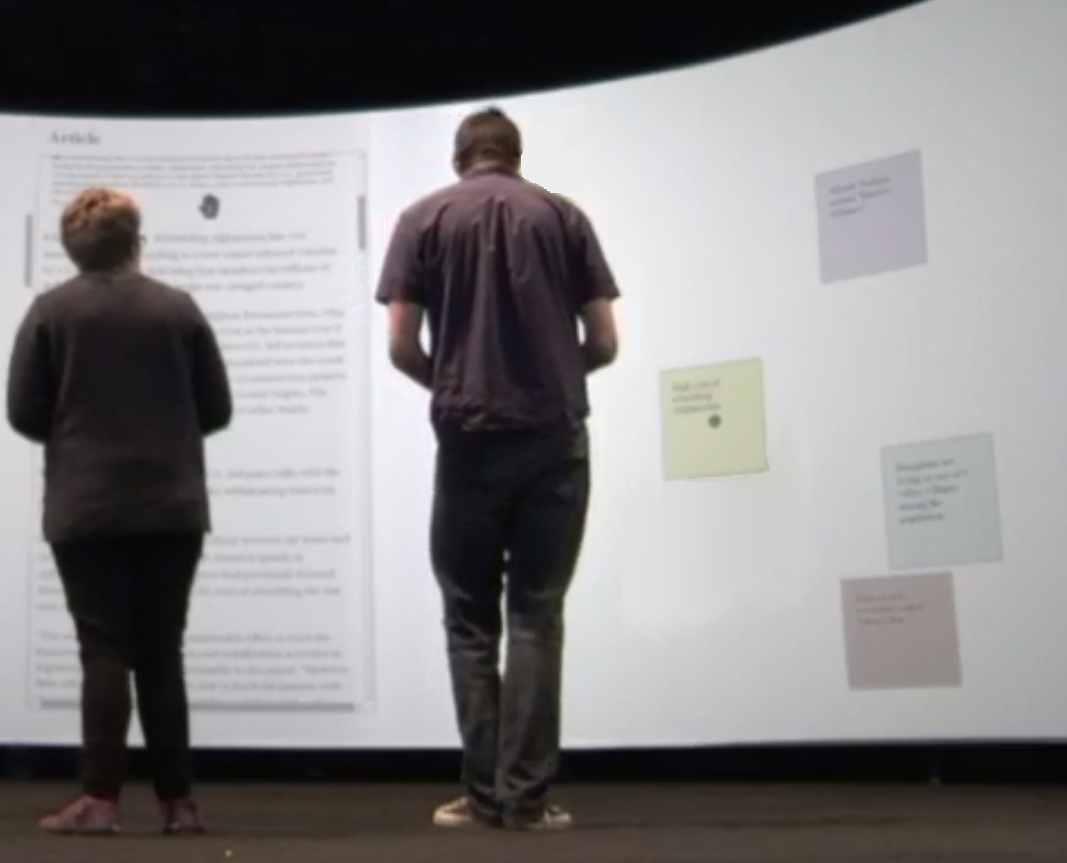
\includegraphics[width=0.7\columnwidth]{chapters/06_planning/figures/intent_sticky_notes.png}
  \caption{Analyst using sticky notes application.}
  \label{fig:intent_sticky_notes}
\end{figure}

We start with grounding our example into a real-world scenario, shown in
Figure~\ref{fig:intent_sticky_notes}. In this scenario, we have two agents once again, \humana\ and
\humanb. There are four notes on the screen, $n1$, $n2$, $n3$, and $n4$ that each have their own color
and location on the screen. Agent \humanb\ is currently pointing at note $n1$ on the screen. We can
axiomatize this set-up as follows:

\begin{center}
\begin{tabular}{ l l l }
    $\holds(\onScreen(n1), 0)$ & 
    $\holds(\position(n1, 50, 50), 0)$ &
    $\holds(\isColor(n1, yellow), 0)$ \\
    $\holds(\onScreen(n2), 0)$ &
    $\holds(\position(n2, 75, 30), 0)$ &
    $\holds(\isColor(n2, purple), 0)$ \\
    $\holds(\onScreen(n3), 0)$ &
    $\holds(\position(n3, 80, 65), 0)$ &
    $\holds(\isColor(n3, blue), 0)$ \\
    $\holds(\onScreen(n4), 0)$ &
    $\holds(\position(n4, 75, 85), 0)$ &
    $\holds(\isColor(n4, red), 0)$ \\
    $\happens(\point(\humanb, n1), 0)$
\end{tabular}
\end{center}

We start first with our example of "Delete that note" as uttered by \humanb. From the conversation-worker,
we receive the \delete\ intent with no further entities. Our orchestrator upon receving the intent then
reaches out to the executor to determine if there are any matching actions to the intent, and receives
the following action, as defined in our STRIPS-style langauge:


\begin{lstlisting}[caption=delete,mathescape=true]
    (define-action delete [(Note ?x)]
        {
            :preconditions [(onScreen ?x)]
            :additions     []
            :deletions     [
                (onScreen ?x)
                $\forall$(y, z) (position ?x y z)
            ]
        }
    )
\end{lstlisting}

From this action, the orchestrator determines that we need a \Note entity to complete the
action, and that we did not receive any such entity from the parsed statement. As such,
the orchestrator then looks to see if it can determine a \Note entity from our context. Here,
it looks through perceived actions of the two agents, scanning in time descending order through
our knowledge base until it finds an action that happened against a note. For our example, it
quickly matches against $\happens(\point(\humanb, n1), 0)$, and given that this action happened
on the same moment as our utterance, then \Note\ $n1$ is deleted. What about had our other agent,
\humana, uttered the statement instead? From our definition of \vicinity\ and its relation to $\perceives$erceiving
as defined in Chapter~\ref{chap:formalizing}, we know that \humana\ has perceived the pointing action
by \humanb. Our orchestrator utilizes that to resolve our intent to the same note in this case.
If both agents were pointing at a note, then the system resolves first to actions committed by that
agent over the ones committed by other agents at the same moment. Finally, the orchestrator
only considers actions that have happened in the recent past (e.g. in the last minute), attempting
to capture the length of attention upon which an agent may give to a particular action or event in
the system. If there is no note that fits our criteria, then the orchestrator issues a request
to the user to clarify which note that they mean.

We now move to our other example of "Delete the yellow note". Similar to above, the orchestrator
gets the same action from the executor and cannot resolve it against any entity in the utterance.
Unlike above however, our utterance contains the \Color\ entity, which is a property of notes and so the
orchestrator then knows that it is additionally looking for a yellow note, or as defined in the
\CEC: $\holds(\isColor(?x, yellow), 0)$. Given this property and the precondition from our action,
our orchestrator generates the query "does there exist a note that is on the screen and is
yellow?" which is formalized as following:

\begin{equation*}
    \exists (\Note\ x) (\holds(\onScreen(x), 0) \land \holds(\isColor(x, yellow), 0))
\end{equation*}

This query is run through \textsf{ShadowProver} as many time as necessary to determine
the candidate set of notes that fit our needs. To accomplish this, for each candidate
returned, we then re-run our query appending a $(x \neq n)$ where $n$ is our discovered
note candidate in the previous step. We keep on appending discovered candidates until the orchestrator
hit a point where \textsf{ShadowProver} can no longer return any matching note. In the case
that the system receives only one note that fits the above query, that note is then removed.
If there are two or more notes, we then utilize a similar algorithm as above, where the
orchestrator scans for actions that relate to any of our candidate notes. If the system
finds any such action within a similar time frame (such as we have in our example), that note
is then used over any other candidate. Similar to above, if there is no way to determine
which note that the user referred to, the system then asks the user to clarify which
note they were referring to.

\begin{figure}
\centering
  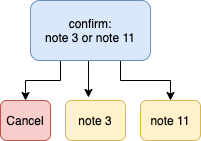
\includegraphics[width=0.3\columnwidth]{chapters/06_planning/figures/intent_resolution_fragment.png}
  \caption{Conditional plan fragment to ask clarification from user.}
  \label{fig:intent_resolution_fragment}
\end{figure}

For cases in which the orchestrator goes back to the user, our system utilizes a similar concept
as employed by Botea et al.~\cite{botea_generating_2019}, where the question to the user
is generated by the orchestrator based on possible candidates and timing, and sets itself up
to expect specific answer types here. For example, let's assume we had two notes that matched
our deletion query. The orchestrator then asks the user for clarification between the two notes
as shown in Figure~\ref{fig:intent_resolution_fragment}, expecting that the response (ignoring
any detected intent) contains one of the notes, or is totally unrelated, thus cancelling the
information request, and continuing as normal. 


%    4. Longer Term Plan Recognition

\section{Plan Recognition for Course Correction}

We finish this chapter with an examination of using plan recognition within our CAIS.
For this, we re-use our scenario from Section~\ref{sect:false_belief}. To re-iterate
the situation, we have two human agents, \humana\ and \humanb, and they are working
in the blocks world domain. Same as before, there are three blocks that are shown
on the screen and they all initially are on the table. This information is
shown below:

\begin{center}
\begin{tabular}{ c c }
    \holds(\on(\ablock, \ctable), 0) & 
    \holds(\clear(\ablock), 0)\\
    \holds(\on(\bblock, \ctable), 0) &     
    \holds(\clear(\bblock), 0)\\
    \holds(\on(\cblock, \ctable), 0) & 
    \holds(\clear(\cblock), 0)
\end{tabular}
\end{center}

This time through, we consider a modified sequence from above, incorporating goals
into the system. On adding a goal to our system, the orchestrator is now set to also
validate all actions taken by agents are in line with the current goals of the system.
Any action that is not valid is then blocked by the orchestrator for proceeding. The
new action sequence is as follows:

\begin{center}
\begin{tabular}{l | l | l}
    $t$ & Event in Natural Language & Event in \CEC\ \\
    \hline
    1 & \humana\ enters and registers with the CAIS & \happens(\register(\humana), 1) \\
    2 & \humanb\ enters and registers with the CAIS & \happens(\register(\humanb), 2) \\
    3 & \humana\ stacks block \ablock\ onto block \bblock\ & \happens(\stack(\ablock, \bblock), 3) \\
    4 & \humanb\ adds goal of block \cblock\ on block \bblock] & \happens(\setGoal(\on(\cblock, \bblock)), 4) \\
    5 & \humanb\ deregisters and leaves the CAIS & \happens(\deregister(\humanb), 5) \\
    6 & \humana\ unstacks block \ablock\ from block \bblock\ & \happens(\unstack(\ablock, \bblock), 6) \\
    7 & \humana\ removes the goal of block \cblock\ on block \bblock\ & \happens(\removeGoal(\on(\cblock, \bblock)), 7) \\
    8 & \humana\ adds the goal of block \ablock\ on block \cblock & \happens(\setGoal(\on(\ablock, \cblock)), 8) \\
    9 & \humana\ stacks block \ablock\ onto block \cblock & \happens(\stack(\ablock, \cblock), 9) \\
    10 & \humanb\ re-enters and registers with CAIS & \happens(\register(\humanb), 10) \\
\end{tabular}\label{table:plan_recognition_actions}
\end{center}

\begin{center}
\begin{tabular}{l | l | l}
    $t$ & Added Fluent & Removed Fluents \\
    \hline
    1 & \holds(\inCAIS(\humana), 1) & \\
    2 & \holds(\inCAIS(\humanb), 2) & \\
    3 & \holds(\on(\ablock, \bblock)), 3) & \makecell[l]{
        \holds(\on(\ablock, \ctable), 2) \\
        \holds(\clear(\bblock), 2) \\
    }\\
    4 & \holds(\goal(\on(\cblock, \bblock)), 4) & \\
    5 & & \holds(\inCAIS(\humanb), 4) \\
    6 & \makecell[l]{
        \holds(\on(\ablock, \ctable), 6) \\
        \holds(\clear(\bblock), 6) \\
    } & \makecell[l]{
        \holds(\on(\ablock, \bblock), 5) \\
    } \\
    7 & & \holds(\goal(\on(\cblock, \bblock)), 6) \\
    8 & \holds(\goal(\on(\ablock, \cblock)), 8) & \\
    9 & \holds(\on(\ablock, \cblock), 9) & \makecell[l]{
        \holds(\on(\ablock, \ctable), 8) \\
        \holds(\clear(\cblock), 8) \\
    } \\
    10 & \holds(\inCAIS(\humanb), 10) & \\
\end{tabular}\label{table:plan_recognition_fluents}
\end{center}

Our diligent \humanb, having returned to the CAIS, sees the state of the world
has moved away from the goal that he set in step 4. He, seeking to achieve that
old goal he still believes is active in the system, attempts to issue the command
"Unstack block A from block C", as he seeks to stack block C onto block B. Our
orchestrator in this case refuses to complete that action as to do so would
move the world away from our goal state of $\on(\ablock, \cblock)$. On refusal
of executing the move, the orchestrator launches into a fallback of plan recognition
over \humanb. The first thing done by the system is to collect the potential goals
that an agent may be following. In this, the system scans through its knowledge base
to find goal addition events that happened within the vicinity of \humanb, giving
us the goals of $\on(\cblock, \bblock)$ and $\on(\ablock, \cblock)$. Next, as per
our definition, the system generates the sequence of actions that would take the
state of the world at the start of step 9 to achieve that goal, giving us an
action sequence. The system finally then takes the action of step 9 and determines
if it within either plan's action sequence. In this case, it finds it as part of
the sequence for the goal of $\on(\cblock, \bblock)$. Taking this information, the
CAIS then scans through its and \humanb's knowledge bases to determine where things
may have gone awry. In this, it determines that \humanb\ did not perceive the goal
state change ate step 6. A summary of this information is then all outputted to the
agents, wherein it shows the agent what plan they were attempting to follow, the plan
that they should have been following, and why they have a difference of information.
This catches the agent up, and their knowledge base is now assumed in regards equal
to that of the room for this sequence.

In addition to utilizing plan recognition above, our CAIS also provides an instantiation
of our property of \textit{Expectation of Usefulness}. This property is
instantiated with the event $e$ being setting a new goal:
$e \equiv \setGoal(\on(\ablock, \cblock)))$:

\begin{footnotesize}
\begin{equation*}
\begin{aligned}
&\perceives\big(\humana, t_8, \happens\big(\setGoal(\on(\ablock,\cblock)), t_{8}\big)\big) \land \perceives\Big(\humana, t_8, \lnot \holds\big(\vicinity(\humanb, setGoal (On(A,C))), t_8\big)\Big) \\
& \hspace{90pt} \rightarrow \believes\Big(\humana, t_{11}, \says\big(\gamma, \humanb, t_{11},
\happens(\setGoal(\on(\ablock,\cblock)), t_8)\big)\Big)
\end{aligned}
\end{equation*}
\end{footnotesize}


% 7. Conclusion
\chapter{CONCLUSION}\label{chap:conclusion}

In this dissertation, we introduced the concept of \textit{cognitive
and immersive systems}, and provided a definition of what constitutes
such a system.  Next, we moved to the architecture, implementation,
and formalization of such a system.  We now look back upon our planned
contributions as enumerated in Section~\ref{sec:contributions}, and
provide some retrospective thoughts pertaining to the work presented
above.  Finally, we share some thoughts regarding future work that
will be developed from the foundational work completed here.

%    1. Thesis Overview
\section{Contributions of the Dissertation, Met}

\begin{enumerate}
    \item \checkmark\ Create a high-level but rigorous and fertile definition for what
        constitutes a CAIS, separating it from a physical robot.

    \begin{itemize}
        \item[] Within this dissertation, we have provided definition for what makes a system
        \textit{cognitive} ($\mathcal{C}$) and what makes it \textit{immersive} ($\mathcal{I}$).
        From these definitions, we can see what an idealized version of a CAIS may look like,
        and indeed, how it a localized physical robot may be able to achieve elements of both
        $\mathcal{C}$ and $\mathcal{I}$, it is not possible to achieve them both fully, or even
        the version presented within this thesis.
    \end{itemize}
  
    \item \checkmark\ Define a framework for how one approaches building a CAIS.
    \begin{itemize}
        \item[] We presented a high-level conceptual framework in
        Section~\ref{sec:cais_architecture} for building out these sorts of systems. Due to the
        high potential number of configurations these systems may be employed into, the framework advocates for
        a modular event-driven system, wherein fusion of sensor data, such as might be needed
        happens downstream from any initial parsing of that sensor. In this purpose, the system
        can handle the loss of a sensor or input mechanism, and that may require the user to
        interact with the system in a different manner, but even there, we can still achieve our
        definition of a CAIS.
    \end{itemize}
    
    \item \checkmark\ Create a real-world implementation of a CAIS, demonstrating at a
  novel level that it:
        \begin{enumerate}
            \item \checkmark\ adapts to a number of potential input mechanisms;
            \item \checkmark\ operates at a true multi-modal and multi-user level; and
            \item \checkmark\ is capable of interacting with and understanding
              third-party content.
        \end{enumerate}
        
    \begin{itemize}
        \item[] Within Chapters~\ref{chap:technology},\ref{chap:reagent},\ref{chap:muifold},
        we created a real world implementation of our CAIS along with several new novel
        technologies to achieve our sub-goals above. From \textit{Reagent}, we demonstrated
        a novel technology that is capable of providing us a functional hook into web-based
        content within the room, understanding what is shown on the page as well as capturing
        and driving user interaction withe content. Additionally, because of its design, Reagent
        can be applied not just to content created specifically for the CAIS, but for most web
        content one might wish to open. Rising from this, we present the \textit{Virtual Mouse API}, wherein
        it allows us to provide all users of our system with their own mouse cursor and ability
        to interact with pages simultaneously with one another. From MUIFOLD, we provide
        a novel framework for building out a UI for cellphones to be used within the CAIS, both
        as a generic pointing device for all users, but also for being able to surface deeper
        interactions with sites that supports it, that would be otherwise impossible on traditional
        pointing devices such as HTC Vive and Kinect cameras. Additionally, due to the modular design
        of all modulars of our system as dictated by our framework, pieces of the work have been
        successfully deployed
        elsewhere~\cite{allen_rensselaer_2019,chabot_collaborative_2020,divekar_humaine_2020}.
    \end{itemize}

    \item \checkmark\ Create a formal definition of a CAIS' implementation and
        its capabilities.
        
    \begin{itemize}
        \item[] In Chapter~\ref{chap:formalizing}, we utilize the \CEC\ drive a formalization of
        our high-level definition. In this way, we provide in exact terms and formulae of the
        cognitive and immersive features discussed in this dissertation. Following this, we also
        provide formalization of the components we utilize in the CAIS, tying together how our
        implementation works and relates to the formalization. Finally, because we have provided
        in exact terms our definitions in this fashion, we were able to derive the property of
        \textit{Expectation of Usefulness}, further separating out a CAIS from a physical robot.
        The formalization, as well as our defined properties and formuale, are to our knowledge
        novel compared to prior work in the space of intelligent or smart rooms.
    \end{itemize}

    \item Utilize the above items to handle tasks of reasoning, planning, and plan recognition
        in and involving a CAIS.
    
    \begin{itemize}
        \item[] Finally, given our implementation and formalization above, we were able to utilize
        these to accomplish tasks in reasoning, planning, and plan recognition, operating at a
        ``theory of mind'' level throughout. Not only that, due to the mechanisms employed, for all
        decisions made by our system, they are fully explainable via a backing proof. Each of these
        demonstrations were deployed and demonstrated in the real-world (albeit against toy domains),
        and that we have shown in highly rigorous terms the power of our cognitive and immersive systems.
    \end{itemize}
\end{enumerate}

%    2. Future Work
\section{Future Work}

We now discuss some promising avenues of future work. We examine two main
thrusts here, within each there are a number of possible extensions and
improvements that may be investigated. The first thrust concerns our
formalization efforts and how we may build upon it. As stated in
Chapter~\ref{chap:formalizing}, we purposely used the \CEC\ to form our
basis, leaving ourselves open to various extensions to it to deal with
more advanced scenarios. Perhaps the biggest extension is to handle the
potentially noisiness of incoming data from sensors and feeding it into
our system. Within this work, we assumed that sensors were providing
perfect information with perfect confidence. In reality, many of the input
mechanisms operate with degrees of confidence on their result. For example,
for each classification that is provided by the conversation-worker, the
Watson Assistant service provides a confidence of its interpretation. For
certain actions, lower allowed confidence levels are fine, such as in the
scenarios presented here, but in more high stakes environments,
the CAIS may need to conduct certain actions only with high confidence and
some with low. To handle this, we look to work by Govindarajulu and
Bringsjord where they incorporate strength factors into a cognitive
calculus~\cite{govindarajulu_strength_2017}. Strength factors can be viewed
as a formalization of part of Chisholm’s rational
belief-fixation~\cite{theory.of.knowledge3.chisholm}. Within the work,
the belief operator is amended such that it has a coefficient, $\sigma$,
such that it ranges from one to five, where beliefs are labelled as (1)
acceptable, (2) some presumption in favor, (3) beyond reasonable doubt,
(4) evident, and (5) certain. An added benefit of this approach is that
the presentation of these strength factors may be easier for understanding
from the layperson versus raw probability values, which people may find
difficult to parse~\cite{kaye_can_1991}.

Another avenue of interest for our formalization efforts is in dealing with 
ethical issues and matters of privacy. When utilizing these collaborative spaces,
as information about specific users grows, a user would have a reasonable
belief that the system will not offer sensitive information to their
colleagues without prior approval. The ``Deontic Cognitive Event
Calculus'' (\DCEC) is an attractive logic to handle these cases, adding in the
deontic operator of obligation on-top of the \CEC. Indeed, Bringsjord et al.
proposes a ``Tenancular AI'' shows the usefulness of the \DCEC\ with regards
to these concerns~\cite{bringsjord_tentacular_2018}. Additionally, the \DCEC\
has been used to model the ethical principals of ``Doctrine of Double
Effect''~\cite{govindarajulu_automating_2017} and ``Doctrine of Triple
Effect''~\cite{peveler_towards_2018}.

The other thrust concerns our technology. First, while we are pleased with
our preliminary results of MUIFOLD and its effectiveness, from it were
identified a number of limitations. The most principle of is in making the
system more robust for how users hold their phones. As identified in
Section~\ref{chap04:limitations} however, we find that users would prefer to
hold their phone at an angle, and then point around that angle. However, our
initial implementation assumed that users were holding their phone flat, which
allowed for a simplification of detecting angle changes only around pitch and
yaw. Implementing roll into the equation would expand usability as we look
to extend our technology into more real-world applications. In that vein,
the evaluation here was preliminary in nature, and a more robust user study
is still required for full evaluation of our technology, especially as it
compares to other mechanisms of relative pointing (e.g. Bluetooth clickers)
and absolute pointers (e.g. Wii remote) both in our laboratory testing, as
well as in real-world usage. Perhaps even more importantly is that the
technology is deployed to real-world usage wherein we may discover additional
issues or strengths only discovered when users engage the technology in a
more natural environment than the Fitts' pointing test.

Finally, the technology and formalization presented here focuses on
co-located environments. This focus was a purposeful one due to the
inherit differences between co-located and distributed that we were
not prepared to address here. The first step towards this would be
working on extending the CAIS implementation we presented here to
a fully distributed set-up, wherein each participant is running their
own transcript-worker, speaker-worker, display-worker, etc., and that
the content to be outputted may be the same, or different per user to
fit their needs, such as the display-workers may have different content
open per user, or the content may be arranged differently. All of this
is to be accounted for within the technology stack, but also must be
incorporated into formalization efforts herein. However, to accomplish this,
our first steps would be on deploying the technology to users for a
given scenario, and perform baseline user studies to understand empirically
real-world usage. From this, we could then better conceptualize and deal
with formalization of the environment, and then bring to bear the fruits
of that formalization effort, such as in intent resolution and plan recognition.



%%%%%%%%%%%%%%%%%%%%%%%%%%%%%%%%%%%%%%%%%%%%%%%%%%%%%%%%%%%%%%%%%%%
%                                                                 %
%                           BIBLIOGRAPHY                          %
%                                                                 %
%%%%%%%%%%%%%%%%%%%%%%%%%%%%%%%%%%%%%%%%%%%%%%%%%%%%%%%%%%%%%%%%%%%

%This method produces a numbered bibliography where the numbers
%correspond to the \cite commands in the text. See the LaTeX manual.
%
\specialhead{REFERENCES}
%\bibliographystyle{abbrv}
\bibliographystyle{IEEEtran}
\bibliography{bib_files/peveler_thesis,bib_files/peveler_misc,bib_files/main72}

% Note that, if you wish, you can use BibTeX to create your bibliography
% from a database. See section 5.6.2 of Memo RPI.110 for information.
%%% Local Variables:
%%% mode: latex
%%% TeX-master: t
%%% End:
 % bibliography
%%%%%%%%%%%%%%%%%%%%%%%%%%%%%%%%%%%%%%%%%%%%%%%%%%%%%%%%%%%%%%%%%%%%
%                                                                 %
%                            APPENDICES                           %
%                                                                 %
%%%%%%%%%%%%%%%%%%%%%%%%%%%%%%%%%%%%%%%%%%%%%%%%%%%%%%%%%%%%%%%%%%%
 
\appendix    % This command is used only once!
%\addcontentsline{toc}{chapter}{APPENDICES}             %toc entry  or:
\addtocontents{toc}{\parindent0pt\vskip12pt APPENDICES} %toc entry, no page #

\chapter{THIS IS AN APPENDIX}
This is a sentence to take up space and look like text.
This is a sentence to take up space and look like text.
This is a sentence to take up space and look like text.
This is a sentence to take up space and look like text.

\section{A Section Heading}

This is how equations are numbered in an appendix:
\begin{equation}
x^2 + y^2 = z^2
\end{equation} 
This is a sentence to take up space and look like text.
This is a sentence to take up space and look like text.
This is a sentence to take up space and look like text.
 
This is a sentence to take up space and look like text.
This is a sentence to take up space and look like text.
This is a sentence to take up space and look like text.
This is a sentence to take up space and look like text.
This is a sentence to take up space and look like text. 

\chapter{THIS IS ANOTHER APPENDIX} 
This is a sentence to take up space and look like text.
This is a sentence to take up space and look like text.
This is a sentence to take up space and look like text.
This is a sentence to take up space and look like text.
This is a sentence to take up space and look like text.
This is a sentence to take up space and look like text.
This is a sentence to take up space and look like text.
This is a sentence to take up space and look like text.
 
 % appendix

\end{document}
